% !TEX root=./adl.tex

\section{Reinforcement Learning for LLMs}

\subsection{Motivation}

% -----------------------------------------------------------------------
\begin{frame}{LLM Training Stages}
  \llmtrainingstages{all}

  \vspace{-0.2em}
  \begin{columns}[T]
    \begin{column}{0.31\textwidth}
      \textbf{\color{blue!60!black}Pretraining}
      \begin{itemize}[nosep]
        \item 1--15T+ tokens
        \item 1000s of GPUs
        \item Weeks to months
        \item Most expensive stage (right now, might change)
      \end{itemize}
    \end{column}
    \begin{column}{0.31\textwidth}
      \textbf{\color{green!50!black}SFT}
      \begin{itemize}[nosep]
        \item 10k--1M+ pairs
        \item 10s of GPUs
        \item Hours to days
        \item Relatively cheap
      \end{itemize}
    \end{column}
    \begin{column}{0.31\textwidth}
      \textbf{\color{orange!70!black}RL}
      \begin{itemize}[nosep]
        \item \textbf{Alignment:}
          \begin{itemize}[nosep]
            \item Preferences / RLHF
            \item 10k--100k prompts
            \item 100s of GPUs, days
          \end{itemize}
        \item \textbf{Reasoning:}
          \begin{itemize}[nosep]
            \item Verifier rewards
            \item 100k+ prompts
            \item 1000s of GPUs, weeks
          \end{itemize}
      \end{itemize}
    \end{column}
  \end{columns}
\end{frame}

% -----------------------------------------------------------------------
\begin{frame}{Human Preference Alignment: Why Not Supervised Learning?}
  \begin{columns}
    \begin{column}{0.55\textwidth}
      \begin{center}
        \begin{tikzpicture}[
          scale=0.75, every node/.style={scale=0.75},
          box/.style={rectangle, draw, rounded corners, fill=blue!8, minimum width=4cm, minimum height=0.7cm, align=center, font=\small},
          resp/.style={rectangle, draw, rounded corners, minimum width=3.2cm, minimum height=0.7cm, align=center, font=\scriptsize},
          arr/.style={-{Stealth[length=4pt]}, thick},
        ]
          \node[box] (prompt) at (0, 3) {Prompt: ``Explain gravity''};
          \node[resp, fill=green!10] (a) at (-2.2, 1.3) {Response A: concise,\\accurate, friendly tone};
          \node[resp, fill=red!10] (b) at (2.2, 1.3) {Response B: verbose,\\slightly condescending};

          \draw[arr] ([xshift=-0.66cm]prompt.south) -- (a.north);
          \draw[arr] ([xshift=0.66cm]prompt.south) -- (b.north);

          \node[font=\small\bfseries, text=green!50!black] at (-2.2, 0.2) {\checkmark\, preferred};
          \node[font=\small\bfseries, text=red!70!black] at (2.2, 0.2) {$\times$\, rejected};

          \node[font=\scriptsize, text=gray, align=center] at (0, -0.5) {Human annotator\\judges overall quality};
        \end{tikzpicture}
      \end{center}
    \end{column}
    \begin{column}{0.45\textwidth}
      \textbf{Why not SFT on the preferred response?}
      \begin{itemize}
        \item SFT requires per-token ground truth
        \item Which tokens made A better than B?
          \begin{itemize}
            \item Was it word choice? Sentence order? Tone? All of them?
          \end{itemize}
        \item Preference is \emphdef{holistic}: correctness, helpfulness, safety, style. It emerges from \emphdef{interaction of all tokens}
        \item Cannot decompose ``A $\succ$ B'' into per-token labels
      \end{itemize}

      \vspace{0.3em}
      \textbf{What SFT on A misses:}
      \begin{itemize}
        \item Ignores the rejected response entirely
        \item Does not learn \emph{what to avoid}
      \end{itemize}
    \end{column}
  \end{columns}
\end{frame}

% -----------------------------------------------------------------------
\begin{frame}{Verifiers: Automated Non-Per-Token Supervision}
  Beyond human preferences, many tasks have \emphdef{automated verifiers} that check outputs without per-token labels:

  \begin{columns}[T]
    \begin{column}{0.48\textwidth}
      \begin{description}
        \item[Math:] ``Solve $\int_0^1 x^2\,dx$''\\
          Verifier: Is the answer $\frac{1}{3}$? \quad {\color{green!50!black}\checkmark} / {\color{red!70!black}$\times$}

        \item[Code:] ``Write a function to sort a list''\\
          Verifier: Run test suite\\
          \texttt{assert sort([3,1,2]) == [1,2,3]}

        \item[Logic:] ``Solve this Sudoku''\\
          Verifier: Do all rows, columns, boxes contain 1--9?
      \end{description}
    \end{column}
    \begin{column}{0.48\textwidth}
      \begin{description}
        \item[Games:] Play a game of Go\\
          Verifier: Did the agent win? $r \in \{-1, +1\}$

        \item[Proof:] ``Prove this theorem''\\
          Verifier: Formal proof checker (e.g.\ Lean)

        \item[Chemistry:] ``Design a molecule with property X''\\
          Verifier: Simulation / wet lab confirms property
      \end{description}

    \end{column}
  \end{columns}

  \vspace{0.3em}
  \begin{tcolorbox}[colback=blue!5, colframe=blue!40, boxrule=0.5pt, arc=2pt, left=4pt, right=4pt, top=2pt, bottom=2pt]
    \begin{itemize}[nosep]
      \item All cases: \emphdef{binary or scalar signal} on the full output. No indication which tokens were good or bad.
      \item Verifiers are cheap, scalable, and do not require human annotation $\Rightarrow$ ideal for RL at scale.
    \end{itemize}
  \end{tcolorbox}
\end{frame}

% -----------------------------------------------------------------------
\begin{frame}{Technical Differences: Dense vs.\ Sparse Supervision}
  \begin{center}
    \begin{tikzpicture}[
      scale=0.8, every node/.style={scale=0.8},
      tok/.style={rectangle, draw, minimum width=0.9cm, minimum height=0.6cm, font=\scriptsize, align=center},
    ]
      % Dense supervision row
      \node[font=\small\bfseries] at (-2.5, 1.5) {SFT:};
      \foreach \i/\w in {0/The, 1/cat, 2/sat, 3/on, 4/the, 5/mat} {
        \node[tok, fill=green!20] (d\i) at (\i*1.1, 1.5) {\w};
        \node[font=\scriptsize, text=green!50!black] at (\i*1.1, 0.8) {$\checkmark$};
      }
      \node[font=\scriptsize, text=gray, align=left] at (8, 1.5) {Loss on\\every token};

      % Sparse supervision row
      \node[font=\small\bfseries] at (-2.5, -0.3) {RL:};
      \node[tok, fill=gray!10] (s0) at (0*1.1, -0.3) {Let};
      \node[tok, fill=gray!10] (s1) at (1*1.1, -0.3) {me};
      \node[tok, fill=gray!10] (s2) at (2*1.1, -0.3) {think};
      \node[tok, fill=gray!10] (s3) at (3*1.1, -0.3) {\ldots};
      \node[tok, fill=gray!10] (s4) at (4*1.1, -0.3) {ans};
      \node[tok, fill=gray!10] (s5) at (5*1.1, -0.3) {42};
      \node[tok, fill=orange!30] (reward) at (6.6, -0.3) {$r$};
      \draw[-{Stealth[length=4pt]}, thick, orange] (s5.east) -- (reward.west);
      \node[font=\scriptsize, text=gray, align=left] at (8, -0.3) {Reward on\\full sequence};

      % Arrow showing credit assignment challenge
      \draw[dashed, orange, thick, -{Stealth[length=4pt]}] (reward.south) -- ++(0, -0.5) -| (s0.south);
      \node[font=\scriptsize, text=orange!70!black, align=center] at (3, -1.5) {Credit assignment: which tokens contributed to the reward?};
    \end{tikzpicture}
  \end{center}

  \begin{description}
    \item[Dense (SFT):] Cross-entropy loss on each token. Easy optimization, but needs per-token ground truth.
    \item[Sparse (RL):] Single reward after full generation. Harder optimization, but works with any sequence-level signal.
  \end{description}
\end{frame}

% -----------------------------------------------------------------------
\begin{frame}{RL for Reasoning: Emergent Chain-of-Thought}
  \emphdef{Chain-of-thought (CoT)}: the model writes intermediate reasoning steps before its final answer,
  spending more \emphdef{test-time compute} to break a hard problem into easier sub-steps.
  \begin{center}
    \begin{tikzpicture}[
      scale=0.78, every node/.style={scale=0.78},
      prompt/.style={rectangle, draw, rounded corners, fill=blue!12, minimum height=0.8cm, align=center, font=\small\bfseries, minimum width=4cm},
      thought/.style={rectangle, draw, rounded corners, fill=gray!8, align=left, font=\scriptsize, text width=4.5cm, inner sep=6pt},
      ans/.style={rectangle, draw, rounded corners, minimum height=0.8cm, align=center, font=\small, minimum width=2.5cm},
      verdict/.style={rectangle, draw, rounded corners, minimum height=0.8cm, align=center, font=\scriptsize, minimum width=3cm},
      arr/.style={-{Stealth[length=5pt]}, thick},
    ]
      % Prompt at top center
      \node[prompt] (prompt) at (0, 0) {``What is $17 \times 23$?''};

      % Left branch: no reasoning, wrong answer
      \node[font=\scriptsize, text=gray] at (-4, -0.8) {no reasoning};
      \node[ans, fill=red!10] (bad) at (-4, -1.6) {$381$};
      \node[verdict, fill=red!15] (vbad) at (-4, -2.8) {$381 \neq 391$ \quad $r = -1$};

      % Right branch: reasoning, correct answer
      \node[thought] (trace) at (4, -1.5) {%
        \texttt{<think>}\\
        $17 \times 20 = 340$\\
        $17 \times 3 = 51$\\
        $340 + 51 = 391$\\
        \texttt{</think>}};
      \node[ans, fill=green!10] (good) at (4, -3.5) {$391$};
      \node[verdict, fill=green!15] (vgood) at (4, -4.7) {$391 = 391$ \quad $r = +1$};

      % Arrows
      \draw[arr, gray] (prompt.south) -- ++(-2.5, -0.4) -- (bad.north);
      \draw[arr] (prompt.south) -- ++(2.5, -0.4) -- (trace.north);
      \draw[arr, gray] (bad.south) -- (vbad.north);
      \draw[arr] (trace.south) -- (good.north);
      \draw[arr] (good.south) -- (vgood.north);

    \end{tikzpicture}
  \end{center}

  \vspace{-0.2em}
  \begin{itemize}[nosep]
    \item The verifier only checks the \emphdef{final answer}, giving no signal on the reasoning steps
    \item Traces that reason are correct more often, so their tokens get reinforced. The model \emphdef{discovers on its own} that reasoning pays off
    \item No human-written CoT labels needed. Longer traces emerge purely from maximizing verifiable reward
  \end{itemize}
\end{frame}

% -----------------------------------------------------------------------
\begin{frame}{Why Reasoning Emerges}
  \begin{columns}
    \begin{column}{0.48\textwidth}
      \textbf{Without RL:}
      \begin{itemize}
        \item SFT model mimics training data
        \item May or may not produce reasoning
        \item No incentive to reason correctly
        \item Reasoning style fixed by data
      \end{itemize}
    \end{column}
    \begin{column}{0.48\textwidth}
      \textbf{With RL + verifier:}
      \begin{itemize}
        \item Correct final answer $\Rightarrow$ positive reward
        \item Responses with reasoning traces tend to be correct more often
        \item RL \emphdef{amplifies} these responses
        \item Reasoning emerges as a \emphdef{byproduct} of reward maximization
      \end{itemize}
    \end{column}
  \end{columns}

  \vspace{0.8em}
  Key insight: We never explicitly train ``think step by step.'' The model learns that \emphdef{reasoning is instrumentally useful} for maximizing reward.

  \vspace{0.3em}
  \sourceref{DeepSeek-R1 \cite{deepseek_r1_2025} demonstrated this at scale with pure RL}
\end{frame}

% -----------------------------------------------------------------------
\begin{frame}{Historical Shift: RL's Growing Role}
  \begin{columns}
    \begin{column}{0.48\textwidth}
      \textbf{Early RLHF (2022--2023):}
      \begin{itemize}
        \item RL as thin alignment layer
        \item Small fraction of total compute
        \item Mainly for safety and style
        \item InstructGPT, ChatGPT, Llama~2
      \end{itemize}
    \end{column}
    \begin{column}{0.48\textwidth}
      \textbf{Modern RL-heavy training (2024+):}
      \begin{itemize}
        \item RL as \emphdef{primary capability driver}
        \item Significant fraction of total compute
        \item Reasoning, math, code via verifiers
        \item DeepSeek-R1, OpenAI o1/o3
      \end{itemize}
    \end{column}
  \end{columns}

  \vspace{0.8em}
  \begin{center}
    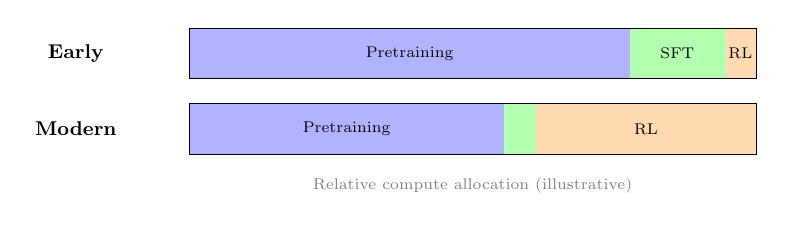
\begin{tikzpicture}[scale=0.8, every node/.style={scale=0.8}]
      % Early bar
      \node[font=\small\bfseries] at (-1.8, 0.8) {Early};
      \fill[blue!30] (0, 0.4) rectangle (7, 1.2);
      \fill[green!30] (7, 0.4) rectangle (8.5, 1.2);
      \fill[orange!30] (8.5, 0.4) rectangle (9, 1.2);
      \draw (0, 0.4) rectangle (9, 1.2);
      \node[font=\scriptsize] at (3.5, 0.8) {Pretraining};
      \node[font=\scriptsize] at (7.75, 0.8) {SFT};
      \node[font=\scriptsize] at (8.75, 0.8) {RL};

      % Modern bar
      \node[font=\small\bfseries] at (-1.8, -0.4) {Modern};
      \fill[blue!30] (0, -0.8) rectangle (5, 0);
      \fill[green!30] (5, -0.8) rectangle (5.5, 0);
      \fill[orange!30] (5.5, -0.8) rectangle (9, 0);
      \draw (0, -0.8) rectangle (9, 0);
      \node[font=\scriptsize] at (2.5, -0.4) {Pretraining};
      \node[font=\scriptsize] at (5.25, -0.4) {};
      \node[font=\scriptsize] at (7.25, -0.4) {RL};

      \node[font=\scriptsize, text=gray] at (4.5, -1.3) {Relative compute allocation (illustrative)};
    \end{tikzpicture}
  \end{center}
\end{frame}

% -----------------------------------------------------------------------
\begin{frame}{Offline vs.\ Online Training}
  \begin{center}
    \begin{tikzpicture}[
      scale=0.82, every node/.style={scale=0.82},
      box/.style={rectangle, draw, rounded corners, minimum width=2.2cm, minimum height=0.8cm, align=center, font=\small},
      data/.style={cylinder, draw, shape border rotate=90, aspect=0.25, minimum height=1cm, minimum width=1.5cm, fill=gray!10, font=\scriptsize, align=center},
      arr/.style={-{Stealth[length=5pt]}, thick},
    ]
      % Separator
      \draw[dashed, gray!50, thick] (0.5, 2.8) -- (0.5, -0.5);

      % --- Offline side ---
      \node[font=\small\bfseries] at (-3.5, 2.5) {Offline (Pretraining \& SFT)};
      \node[data] (fixdata) at (-5.5, 1) {Fixed\\Dataset};
      \node[box, fill=blue!15] (model1) at (-1.8, 1) {Model};
      \draw[arr] (fixdata) -- (model1) node[midway, above, font=\scriptsize] {sample batch};

      % --- Online side ---
      \node[font=\small\bfseries] at (5.5, 2.5) {Online (RL)};
      \node[box, fill=orange!15] (model2) at (3.2, 1) {Model};
      \node[box, fill=yellow!10] (env) at (7.8, 1) {Reward};
      \draw[arr] (model2.north) to[bend left=35] node[midway, above, font=\scriptsize] {generate} (env.north);
      \draw[arr] (env.south) to[bend left=35] node[midway, below, font=\scriptsize] {reward} (model2.south);
    \end{tikzpicture}
  \end{center}

  \vspace{-0.2em}
  \begin{columns}[T]
    \begin{column}{0.47\textwidth}
      \begin{itemize}[nosep]
        \item Data collected once, training iterates over it
        \item Model does not influence training data
        \item Dense supervision (per-token loss)
        \item \emphdef{Distribution mismatch}: model trains on states the \emph{teacher/data} visits, not states the \emph{model} will encounter
        \item Compounding error: early mistakes lead to unseen states $\Rightarrow$ model diverges
      \end{itemize}
    \end{column}
    \begin{column}{0.47\textwidth}
      \begin{itemize}[nosep]
        \item Model generates its own training data
        \item Learns from states \emphdef{it actually visits} at inference time
        \item Sparse supervision (reward on full sequence)
        \item No distribution mismatch
        \item Can \emphdef{explore} and discover novel solutions
        \item Non-stationary, harder to stabilize
      \end{itemize}
    \end{column}
  \end{columns}
\end{frame}

% -----------------------------------------------------------------------
\begin{frame}{Offline vs.\ Online: Chess Analogy}
  \begin{columns}[T]
    \begin{column}{0.48\textwidth}
      \textbf{Offline (SFT / distillation):}
      \begin{itemize}
        \item Like \emphdef{watching a grandmaster} play chess
        \item You see brilliant moves, but in board positions \emph{you} would never reach
        \item Dense signal (learn from every move) but in the \emphdef{wrong distribution}
      \end{itemize}
    \end{column}
    \begin{column}{0.48\textwidth}
      \textbf{Online (RL):}
      \begin{itemize}
        \item Like \emphdef{playing chess yourself} with no coach
        \item You experience your own board positions
        \item Sparse signal (only win/loss at the end) but in the \emphdef{right distribution}
      \end{itemize}
    \end{column}
  \end{columns}

  \vspace{0.8em}
  \begin{tcolorbox}[colback=blue!5, colframe=blue!40, boxrule=0.5pt, arc=2pt, left=4pt, right=4pt, top=2pt, bottom=2pt]
    \textbf{Ideal:} A grandmaster watches \emph{you} play and comments on each move $=$ \emphdef{on-policy distillation} (dense supervision on student-generated data).
  \end{tcolorbox}
\end{frame}

% -----------------------------------------------------------------------
\begin{frame}{Remarks}
  \begin{itemize}\largesep
    \item Attending a full RL course is advised
    \item We will distill a big field into a short excursion
    \item Wonderful theory and intricate algorithms; we scratch the surface
    \item Recommended resources:
      \begin{itemize}
        \item Sutton \& Barto, \emph{Reinforcement Learning: An Introduction}, 2nd ed.~\cite{sutton2018rl}
        \item David Silver's RL lecture series~\cite{silver2015rl}
      \end{itemize}
  \end{itemize}
\end{frame}

\subsection{RL Introduction}

% -----------------------------------------------------------------------
\begin{frame}{RL Intro}
  \begin{center}
    \begin{tikzpicture}[
      scale=0.7, every node/.style={scale=0.7},
      arr/.style={-{Stealth[length=6pt]}, thick, gray!70},
    ]
      % Agent image (left)
      \node[inner sep=0pt] (agent) at (0, 0)
        {
\includegraphics[height=1.8cm]{images/RL_robot_agent.png}};
      \node[font=\small\bfseries, above=2pt of agent] {AGENT};

      % Environment image (right)
      \node[inner sep=0pt] (env) at (6, 0)
        {
\includegraphics[height=1.8cm]{images/RL_world_environment.png}};
      \node[font=\small\bfseries, above=2pt of env] {ENVIRONMENT};

      % Top arrow: agent -> environment (action)
      \draw[arr] (agent.north east) to[bend left=28]
        node[above, font=\scriptsize, align=center, text=black]
        {State $s \in \mathcal{S}$\\Take action $a \in \mathcal{A}$}
        (env.north west);

      % Bottom arrow: environment -> agent (reward + new state)
      \draw[arr] (env.south west) to[bend left=28]
        node[below, font=\scriptsize, align=center, text=black]
        {Get reward $r$\\New state $s' \in \mathcal{S}$}
        (agent.south east);
    \end{tikzpicture}
  \end{center}

  \vspace{-0.5em}
  \begin{columns}[T]
    \begin{column}{0.33\textwidth}
      \textbf{Environment:}
      \begin{itemize}[nosep]
        \item State $s \in \mathcal{S}$
        \item Transition: $P(s' \mid s, a)$
        \item Reward: $R(s, a, s')$
      \end{itemize}

      \vspace{0.2em}
      \textbf{Agent:}
      \begin{itemize}[nosep]
        \item Policy: $a \sim \pi(\cdot \mid s)$
      \end{itemize}
    \end{column}
    \begin{column}{0.30\textwidth}
      \textbf{Objective:}
      \[
        \max_\pi \E\!\left[\sum_{t=0}^{T} \gamma^t r_t\right]
      \]
      $\gamma \in [0,1]$: discount factor
    \end{column}
    \begin{column}{0.35\textwidth}
      \textbf{Trajectory loop:}
      \begin{center}
        \begin{tikzpicture}[
          scale=0.6, every node/.style={scale=0.6},
          loopstep/.style={rectangle, draw, rounded corners, fill=blue!8, minimum height=0.5cm, font=\scriptsize, align=center},
          arr/.style={-{Stealth[length=3pt]}, thick},
        ]
          \node[loopstep] (s) at (0, 0) {observe $s_t$};
          \node[loopstep] (a) at (0, -1.2) {select $a_t \sim \pi$};
          \node[loopstep] (r) at (0, -2.4) {get $r_t, s_{t+1}$};
          \node[loopstep] (store) at (0, -3.6) {$t \leftarrow t{+}1$};
          \draw[arr] (s) -- (a);
          \draw[arr] (a) -- (r);
          \draw[arr] (r) -- (store);
          \draw[arr] (store.east) -- ++(0.6,0) |- (s.east);
        \end{tikzpicture}
      \end{center}
    \end{column}
  \end{columns}
  \sourceref{Images: Lilian Weng, \url{https://lilianweng.github.io/posts/2018-02-19-rl-overview/}}
\end{frame}

% -----------------------------------------------------------------------
\begin{frame}{RL Toy Example}
  \begin{columns}
    \begin{column}{0.52\textwidth}
      \begin{center}
        \gridworld{0.72}
      \end{center}
    \end{column}
    \begin{column}{0.46\textwidth}
      \textbf{Grid world:}
      \begin{description}[nosep]
        \item[State:] Cell position $(x, y)$
        \item[Actions:] $\{\uparrow, \downarrow, \leftarrow, \rightarrow\}$
        \item[Obstacles:] Cannot be entered (black)
      \end{description}

      \vspace{0.4em}
      \textbf{Rewards:}
      \begin{itemize}[nosep]
        \item $-1$ per step (empty cell)
        \item $-5$ for trap cells {\color{red!70!black}(red)}
        \item $+100$ for reaching the goal {\color{cyan!50!black}(cyan)}
      \end{itemize}
      Trajectory ends upon reaching goal or trap.

      \vspace{0.4em}
      \textbf{Agent} {\color{red!70!black}($\bullet$)}: Follows policy $a_t \sim \pi(\cdot \mid s_t)$

      \vspace{0.3em}
      \textbf{Two trajectories} ($\gamma = 1$):
      \begin{itemize}[nosep]
        \item {\color{green!50!black}$\tau_1$}: 12 steps $+$ goal\\
          $R(\tau_1) = 12 \cdot ({-}1) + 100 = 88$
        \item {\color{red!60}$\tau_2$}: 5 steps $+$ trap\\
          $R(\tau_2) = 5 \cdot ({-}1) + ({-}5) = {-}10$
      \end{itemize}
    \end{column}
  \end{columns}
\end{frame}

% -----------------------------------------------------------------------
\begin{frame}{RL Setting for LLMs}
  \begin{center}
    \begin{tikzpicture}[
      scale=0.82, every node/.style={scale=0.82},
      tok/.style={rectangle, draw, minimum width=1cm, minimum height=0.7cm, font=\scriptsize, align=center},
      brace/.style={decorate, decoration={brace, amplitude=5pt}},
      bracebelow/.style={decorate, decoration={brace, amplitude=5pt, mirror}},
    ]
      % Prompt tokens
      \node[tok, fill=blue!15] (t0) at (0, 0) {What};
      \node[tok, fill=blue!15] (t1) at (1.1, 0) {is};
      \node[tok, fill=blue!15] (t2) at (2.2, 0) {2+3};
      \node[tok, fill=blue!15] (t3) at (3.3, 0) {?};
      % Response tokens
      \node[tok, fill=orange!15] (t4) at (4.7, 0) {The};
      \node[tok, fill=orange!15] (t5) at (5.8, 0) {answer};
      \node[tok, fill=orange!15] (t6) at (6.9, 0) {is};
      \node[tok, fill=orange!15] (t7) at (8.0, 0) {5};
      % Reward
      \node[rectangle, draw, rounded corners, fill=green!20, minimum width=0.8cm, minimum height=0.7cm, font=\scriptsize\bfseries] (rew) at (9.3, 0) {$r$};
      \draw[-{Stealth[length=4pt]}, thick, green!50!black] (t7.east) -- (rew.west);

      % States: braces below spanning from prompt start to current token
      \draw[bracebelow, thick, blue!60] (t0.south west) ++(0,-0.1) -- ++(4.3,0)
        node[midway, below=6pt, font=\scriptsize, text=blue!60] {$s_0$};
      \draw[bracebelow, thick, blue!60] (t0.south west) ++(0,-0.55) -- ++(5.7,0)
        node[midway, below=6pt, font=\scriptsize, text=blue!60] {$s_1$};
      \draw[bracebelow, thick, blue!60] (t0.south west) ++(0,-1.0) -- ++(6.8,0)
        node[midway, below=6pt, font=\scriptsize, text=blue!60] {$s_2$};

      % Actions: braces above for each generated token
      \draw[brace, thick, orange!70!black] (t4.north west) ++(0,0.1) -- ++(1.0,0)
        node[midway, above=6pt, font=\scriptsize, text=orange!70!black] {$a_0$};
      \draw[brace, thick, orange!70!black] (t5.north west) ++(0,0.1) -- ++(1.0,0)
        node[midway, above=6pt, font=\scriptsize, text=orange!70!black] {$a_1$};
      \draw[brace, thick, orange!70!black] (t6.north west) ++(0,0.1) -- ++(1.0,0)
        node[midway, above=6pt, font=\scriptsize, text=orange!70!black] {$a_2$};
      \draw[brace, thick, orange!70!black] (t7.north west) ++(0,0.1) -- ++(1.0,0)
        node[midway, above=6pt, font=\scriptsize, text=orange!70!black] {$a_3$};

      % Labels
      \node[font=\scriptsize, text=blue!60] at (1.65, 1.0) {\textbf{prompt}};
      \node[font=\scriptsize, text=orange!70!black] at (6.35, 1.0) {\textbf{response (generated)}};
    \end{tikzpicture}
  \end{center}

  \vspace{0.3em}
  \begin{description}
    \item[Agent:] The LLM itself
    \item[State $s_t$:] All tokens so far (prompt + response until now)
    \item[Action $a_t$:] Next token to generate
    \item[Policy:] $a_t \sim \pi_\theta(\cdot \mid s_t)$: softmax distribution over vocabulary
    \item[Reward $r$:] Scalar signal after full response (verifier or preference model)
  \end{description}
\end{frame}


\subsection{Reward Model}

% -----------------------------------------------------------------------
\begin{frame}{Reward for LLMs}
  \begin{itemize}
    \item Assigning exact reward to text is hard, but \emphdef{comparing two responses} is often easy
    \item Train reward model on pairs: given $(x, y_w)/(x, y_l)$, enforce $r(x, y_w) > r(x, y_l)$
  \end{itemize}

  \begin{tcolorbox}[colback=green!3, colframe=green!40!black, boxrule=0.5pt, arc=2pt, title={\small Bradley-Terry Model}, fonttitle=\bfseries]
    Probability that $y_w$ is preferred over $y_l$:
    \[
      P(y_w \succ y_l) = \frac{\exp r(x, y_w)}{\exp r(x, y_w) + \exp r(x, y_l)} = \sigma\bigl(r(x, y_w) - r(x, y_l)\bigr)
    \]

    \vspace{-0.5em}
    MLE on comparison data gives the \emphdef{reward loss}:
    \[
      \mathcal{L} = -\sum_{(y_w, y_l)} \log \sigma\bigl(r(x, y_w) - r(x, y_l)\bigr)
    \]
  \end{tcolorbox}

  \vspace{0.2em}
  \begin{itemize}[nosep]
    \item $r(x, y_w) > r(x, y_l) \Rightarrow$ sigmoid $> 0.5 \Rightarrow$ loss is small
    \item $r(x, y_w) < r(x, y_l) \Rightarrow$ sigmoid $< 0.5 \Rightarrow$ loss is large
  \end{itemize}
\end{frame}

% -----------------------------------------------------------------------
\begin{frame}{Reward Model for LLMs}
  \begin{center}
    \begin{tikzpicture}[
      scale=0.75, every node/.style={scale=0.75},
      tok/.style={rectangle, draw, rounded corners, fill=red!15, minimum width=0.9cm, minimum height=0.6cm, font=\scriptsize, align=center},
      hs/.style={rectangle, draw, rounded corners, fill=red!10, minimum width=0.9cm, minimum height=0.6cm, font=\scriptsize, align=center},
      transformer/.style={rectangle, draw, rounded corners, fill=purple!20, minimum height=1.5cm, align=center, font=\small},
      linear/.style={rectangle, draw, rounded corners, fill=purple!40, minimum height=0.5cm, align=center, font=\scriptsize},
      arr/.style={-{Stealth[length=4pt]}, thick},
    ]
      % Input tokens
      \foreach \i/\w in {0/What, 1/is, 2/grav, 3/ity, 4/?, 5/It, 6/pulls, 7/things} {
        \node[tok] (t\i) at (\i*1.15, 0) {\w};
      }
      \node[font=\scriptsize, text=gray, anchor=east] at (-0.8, 0) {Input tokens:};

      % Transformer block
      \node[transformer, minimum width=9.2cm] (trans) at (3.5*1.15, 1.8) {Transformer};

      % Arrows from tokens to transformer
      \foreach \i in {0,...,7} {
        \draw[arr, gray!60] (t\i.north) -- (t\i.north |- trans.south);
      }

      % Hidden states
      \foreach \i in {0,...,7} {
        \node[hs] (h\i) at (\i*1.15, 3.3) {$h_{\i}$};
      }
      \node[font=\scriptsize, text=gray, anchor=east] at (-0.8, 3.3) {Hidden states:};

      % Arrows from transformer to hidden states
      \foreach \i in {0,...,7} {
        \draw[arr, gray!60] (h\i.south |- trans.north) -- (h\i.south);
      }

      % Highlight last hidden state
      \node[hs, fill=orange!30, thick] (hlast) at (7*1.15, 3.3) {$h_7$};

      % Linear layer on last hidden state
      \node[linear] (lin) at (7*1.15, 4.3) {Linear $(d \to 1)$};
      \draw[arr] (hlast.north) -- (lin.south);

      % Reward output
      \node[font=\small\bfseries] (reward) at (7*1.15, 5.1) {Reward $r$};
      \draw[arr] (lin.north) -- (reward.south);

      % Annotation
      \draw[dashed, orange, thick] (7*1.15 - 0.65, 2.95) rectangle (7*1.15 + 0.65, 5.4);
      \node[font=\tiny, text=orange!70!black, anchor=west] at (7*1.15 + 0.8, 4.3) {last token only};
    \end{tikzpicture}
  \end{center}

  \vspace{-0.3em}
  \begin{itemize}[nosep]
    \item Start from a pretrained LLM, replace the output head with a \emphdef{scalar linear layer}
    \item Feed prompt $+$ response, take the \emphdef{last token's hidden state} $\to$ linear $\to$ reward $r \in \mathbb{R}$
    \item Train on human comparison data using the Bradley-Terry loss
  \end{itemize}
\end{frame}

\subsection{Policy Gradient}

% -----------------------------------------------------------------------
\begin{frame}{Loss on Trajectories}
  \textbf{Notation:}
  \begin{itemize}[nosep]
    \item Trajectory $\tau = (s_0, a_0, r_0, \ldots, s_T, a_T, r_T)$, \quad return $R(\tau) = \sum_{t=0}^{T} \gamma^t r_t$
    \item $\pi_\theta(a_t \mid s_t)$: policy: the LLM with parameters $\theta$, outputs next-token distribution
    \item $\rho_0(s_0)$: distribution over initial states (e.g.\ prompt distribution)
    \item $P(s_{t+1} \mid s_t, a_t)$: environment transition: deterministic for LLMs (append token)
  \end{itemize}

  \vspace{0.3em}
  \textbf{Goal:} Find parameters $\theta$ that maximize the expected return:
  \[
    \theta^* = \argmax_\theta J(\theta), \qquad J(\theta) = \E_{\tau \sim \pi_\theta}[R(\tau)] = \int P(\tau \mid \theta) \, R(\tau) \, d\tau
  \]
  $J(\theta)$: expected return over all trajectories sampled from the current policy $\pi_\theta$.

  \vspace{0.3em}
  \textbf{Probability of trajectory:}
  \[
    P(\tau \mid \theta) = \rho_0(s_0) \prod_{t=0}^{T-1} P(s_{t+1} \mid s_t, a_t) \, \pi_\theta(a_t \mid s_t)
  \]
\end{frame}

% -----------------------------------------------------------------------
\begin{frame}{Policy Gradient Optimization}
  Parametrize $\pi_\theta$ via weights of LLM. Update: $\theta_{t+1} \leftarrow \theta_t + \alpha \nabla_\theta J(\theta)\big|_{\theta_k}$

  \vspace{0.3em}
  \textbf{Why is optimizing $J(\theta)$ hard?}
  \begin{itemize}
    \item \textbf{Integral over trajectories:} $J(\theta) = \int P(\tau \mid \theta) R(\tau)\, d\tau$. Cannot enumerate; must \emphdef{sample}
    \item \textbf{Non-differentiable environment:} $P(s_{t+1} \mid s_t, a_t)$ and $R(\tau)$ are black boxes. Cannot backpropagate through them
    \item \textbf{Non-stationarity:} Data distribution $P(\tau \mid \theta)$ \emphdef{depends on the policy} being optimized, changing with every update, old samples become stale
    \item \textbf{High variance:} Small policy changes can lead to very different trajectories $\Rightarrow$ gradient estimates are noisy
    \item \textbf{Temporal correlation:} Tokens within a trajectory are highly correlated, violating i.i.d.\ assumptions of standard SGD
    \item \textbf{Sparse reward:} Often only a single reward at the end of a full sequence. Credit assignment across hundreds of tokens
  \end{itemize}

  \vspace{0.3em}
  $\Rightarrow$ Need specialized techniques: policy gradient theorem, variance reduction, importance sampling.
\end{frame}

% -----------------------------------------------------------------------
\begin{frame}{Policy Gradient Theorem: Derivation}
  \begin{theorem}[Policy Gradient]
    For $J(\theta) = \E_{\tau \sim \pi_\theta}[R(\tau)]$,
    \[
      \nabla_\theta J(\theta) = \E_{\tau \sim \pi_\theta}\!\left[\nabla_\theta \log P(\tau \mid \theta) \, R(\tau)\right].
    \]
  \end{theorem}

  \vspace{0.3em}
  \textbf{Proof:}
  \begin{align*}
    \nabla_\theta J(\theta) &= \nabla_\theta \E_{\tau \sim \pi_\theta}[R(\tau)] \\
    &= \nabla_\theta \int P(\tau \mid \theta) \, R(\tau) \, d\tau && \text{expand expectation} \\
    &= \int \nabla_\theta P(\tau \mid \theta) \, R(\tau) \, d\tau && \text{gradient under integral} \\
    &= \int P(\tau \mid \theta) \, \nabla_\theta \log P(\tau \mid \theta) \, R(\tau) \, d\tau && \text{log-derivative trick} \\
    &= \E_{\tau \sim \pi_\theta}\!\left[\nabla_\theta \log P(\tau \mid \theta) \, R(\tau)\right] && \text{back to expectation}
  \end{align*}

  \textbf{Log-derivative trick:} $\nabla_\theta P(\tau \mid \theta) = P(\tau \mid \theta) \, \nabla_\theta \log P(\tau \mid \theta)$

  \vspace{0.3em}
  Key insight: We no longer need to differentiate through the environment, only through $\log P(\tau \mid \theta)$.
\end{frame}

% -----------------------------------------------------------------------
\begin{frame}{Policy Gradient Theorem: Final Form}
  The trajectory probability factorizes into initial state, transitions, and actions:
  \[
    P(\tau \mid \theta) = \rho_0(s_0) \prod_{t} P(s_{t+1} \mid s_t, a_t) \, \pi_\theta(a_t \mid s_t)
  \]
  Taking the log turns the product into a sum:
  \[
    \log P(\tau \mid \theta) = \log \rho_0(s_0) + \sum_{t} \log P(s_{t+1} \mid s_t, a_t) + \sum_{t} \log \pi_\theta(a_t \mid s_t)
  \]

  \vspace{0.3em}
  Only $\log \pi_\theta$ depends on $\theta$, so environment terms vanish under $\nabla_\theta$:

  \[
    \boxed{\nabla_\theta J(\theta) = \E_{\tau \sim \pi_\theta}\!\left[\sum_{t=0}^{T} \nabla_\theta \log \pi_\theta(a_t \mid s_t) \, R(\tau)\right]}
  \]

  \begin{itemize}
    \item $\nabla_\theta \log \pi_\theta(a_t \mid s_t)$: gradient of log-probability of action taken, computable via backprop through the LLM
    \item $R(\tau)$: return of the trajectory (scalar, no gradient needed)
    \item Approximate expectation by \emphdef{sampling trajectories}: $\nabla_\theta J(\theta) \approx \frac{1}{|D|} \sum_{\tau \in D} \sum_{t=0}^{T} \nabla_\theta \log \pi_\theta(a_t \mid s_t) \, R(\tau)$
  \end{itemize}
\end{frame}

% -----------------------------------------------------------------------
\begin{frame}{REINFORCE Algorithm}
  \begin{algorithm}[H]
  \small
  \caption{REINFORCE}
  \KwInput{Policy $\pi_\theta$ (the LLM), reward model $R$, prompt dataset $\mathcal{P}$, batch size $B$, learning rate $\alpha$}
  Initialize policy parameters $\theta$\;
  \For{$k = 0$ \KwTo $K-1$}{
    \tcp{one on-policy update: rollouts use current $\theta$}
    Sample a minibatch of prompts $\{x^{(i)}\}_{i=1}^{B} \sim \mathcal{P}$\;
    \For{$i = 1$ \KwTo $B$}{
      \tcp{autoregressive rollout of the response}
      $s_0 \leftarrow x^{(i)}$\;
      \For{$t = 0, 1, 2, \dots$}{
        $a_t \sim \pi_\theta(\cdot \mid s_t)$ \tcp*{sample next token}
        $s_{t+1} \leftarrow s_t \oplus a_t$ \tcp*{append token to context}
        \lIf{$a_t = \texttt{[EOS]}$ \textbf{or} $t = T_{\max}$}{\textbf{break}}
      }
      $\tau_i \leftarrow (x^{(i)}, a_0, a_1, \dots, a_{T_i-1})$\;
      $R(\tau_i) \leftarrow$ score of full response with reward model / verifier\;
    }
    \textbf{Estimate policy gradient:}\;
    \Indp
      $\hat{g} = \frac{1}{B} \sum_{i=1}^{B} \sum_{t=0}^{T_i-1} \nabla_\theta \log \pi_\theta(a_t \mid s_t) \, R(\tau_i)$\;
    \Indm
    \textbf{Update:} $\theta \leftarrow \theta + \alpha \, \hat{g}$\;
  }
  \end{algorithm}

  \vspace{0.3em}
  \begin{description}[nosep]
    \item[Outer loop $k$:] Each iteration is one gradient step on $\theta$. Rollouts are \emphdef{on-policy}: regenerated from the current $\pi_\theta$ every iteration, then discarded.
    \item[State / action:] $s_t = $ prompt $+$ tokens generated so far; action $a_t = $ next token. Continuing a trajectory $=$ autoregressive decoding.
    \item[Reward:] One scalar $R(\tau_i)$ per finished response (reward model or verifier); every token in the response shares it.
  \end{description}
\end{frame}

% -----------------------------------------------------------------------
\begin{frame}{REINFORCE: Problems in Practice}
  \begin{itemize}[nosep]
    \item \emphdef{High variance:} the gradient estimator has large variance, so it needs many samples to converge.
    \item \emphdef{No baseline:} uses absolute rewards rather than relative performance, wasting information about which actions are better than average.
    \item \emphdef{Sample inefficiency:} strictly on-policy, each rollout is used for a single update then discarded.
    \item \emphdef{Instability:} large, noisy steps can collapse the policy; no mechanism limits how far $\theta$ moves per update.
  \end{itemize}
\end{frame}


\subsection{Reducing Variance}

% -----------------------------------------------------------------------
\begin{frame}{Why REINFORCE Has High Variance}
  \begin{itemize}[nosep]
    \item Each rollout: unbiased estimate $g_i = R_i\,\nabla_\theta\log\pi_\theta(a_i\mid s)$, $\E[g_i] = \nabla_\theta J$.
    \item Sample estimates (grey) scatter around the true gradient (red); their \emph{average is the red arrow} in both panels.
    \item Wider scatter $\Rightarrow$ more rollouts needed to average out the noise.
  \end{itemize}
  \begin{center}
  \begin{tikzpicture}[
      scale=0.46, every node/.style={scale=0.46},
      samplearr/.style={-{Stealth[length=4pt]}, gray!55, line width=0.6pt},
      truearr/.style={-{Stealth[length=8pt]}, red!80!black, line width=1.8pt},
    ]
    % Mean (true gradient) tip: length 3.0 at 72 degrees (points up), identical in both panels.
    \coordinate (O)  at (0,0);
    \coordinate (M)  at (72:3.0);
    \coordinate (O2) at (11,0);
    \coordinate (M2) at ($(11,0)+(72:3.0)$);

    % Samples drawn as symmetric +/- noise pairs about the mean tip:
    % for every base direction (a:r) we draw a tip at M+(a:r) AND at M+(a+180:r),
    % so the two cancel and the average of all tips is EXACTLY M (the red arrow).
    % LEFT PANEL: high variance -- large noise radii
    \foreach \a/\r in {10/1.5, 45/1.25, 80/1.55, 120/1.15, 155/1.4, 205/1.0, 250/1.45} {
      \draw[samplearr] (O) -- ($(M)+(\a:\r)$);
      \draw[samplearr] (O) -- ($(M)+(\a+180:\r)$);
    }
    \draw[truearr] (O) -- (M);
    \fill[black] (O) circle (2.2pt);

    % RIGHT PANEL: low variance -- small noise radii (same directions, ~1/3 the spread)
    \foreach \a/\r in {10/0.5, 45/0.42, 80/0.52, 120/0.38, 155/0.47, 205/0.34, 250/0.5} {
      \draw[samplearr] (O2) -- ($(M2)+(\a:\r)$);
      \draw[samplearr] (O2) -- ($(M2)+(\a+180:\r)$);
    }
    \draw[truearr] (O2) -- (M2);
    \fill[black] (O2) circle (2.2pt);

    % titles
    \node[align=center] at (0,5.0)  {\textbf{High variance}};
    \node[align=center] at (11,5.0) {\textbf{Low variance}};

    % captions
    \node[align=center, gray!50!black] at (0,-1.3)  {\footnotesize same mean, wide scatter\\[-2pt]$\Rightarrow$ noisy average};
    \node[align=center, gray!50!black] at (11,-1.3) {\footnotesize same mean, tight scatter\\[-2pt]$\Rightarrow$ stable average};

    % theta labels
    \node[below left=-2pt] at (O)  {$\theta$};
    \node[below left=-2pt] at (O2) {$\theta$};

    % legend for true gradient
    \draw[truearr] (2.8,-0.6) -- ++(0:0.9);
    \node[anchor=west, red!80!black] at (3.8,-0.6) {\footnotesize true gradient $\E[g]=\nabla_\theta J$ (same in both)};
  \end{tikzpicture}
  \end{center}

  \begin{itemize}[nosep]
    \item Both are unbiased: only the \emph{spread} of the estimator differs, not what it converges to.
    \item Next: what exactly drives that spread, and how to shrink it without touching the mean.
  \end{itemize}
\end{frame}

% -----------------------------------------------------------------------
\begin{frame}{What Drives the Variance? Magnitude, Not Spread of $R$}
  Write the score $s = \nabla_\theta\log\pi_\theta(a\mid s)$, so a single-sample gradient is $g = R\,s$. The score is zero-mean,
  \[
    \E[s]=\sum_a \pi_\theta\,\tfrac{\nabla_\theta\pi_\theta}{\pi_\theta}=\nabla_\theta\sum_a\pi_\theta=\nabla_\theta 1 = 0,
    \qquad\text{so}\qquad
    \mathrm{Var}(g) = \E[R^2 s^2] - \underbrace{(\E[R\,s])^2}_{=\,(\nabla_\theta J)^2}.
  \]
  \begin{itemize}[nosep]
    \item Noise is governed by the \emph{raw second moment} $\E[R^2 s^2]$: the reward \emph{magnitude} $R$, weighted by $s^2\ge 0$, drives the spread, not how much $R$ fluctuates about its own mean.
    \item \textbf{Shift test.} Offset $R\to R+c$. The mean is untouched, $\E[(R+c)s]=\E[Rs]+c\,\E[s]=\E[Rs]$, so the optimum is unchanged, yet
      \[
        \E[(R+c)^2 s^2] = \E[R^2 s^2] + 2c\,\E[R s^2] + c^2\,\E[s^2]
      \]
      grows quadratically in $c$: pure offset, more noise, same solution.
    \item So $\mathrm{Var}(R)$ (shift-invariant) is \emph{not} the culprit. Large all-positive returns (big $\E[R^2]$, small $\mathrm{Var}(R)$) are the worst case, e.g.\ every rollout gets reward $\approx +100$.
  \end{itemize}

  \vspace{0.4em}
  \textbf{Two ways to shrink $\E[R^2 s^2]$ while keeping the mean.} Both leave $\nabla_\theta J$ unchanged (each removed piece has zero expectation against $s$):
  \begin{description}[nosep,leftmargin=!,labelwidth=\widthof{\textbf{Baseline}}]
    \item[\textbf{Reward-to-go}] drop reward earned \emph{before} an action: it is uncorrelated with that action's score, so it only adds noise.
    \item[\textbf{Baseline}] subtract a reference level $b(s)$: recenter $R$ so its second moment collapses toward its \emph{variance}, killing the offset term above.
  \end{description}
\end{frame}

% -----------------------------------------------------------------------
\begin{frame}{REINFORCE Gradient: Reducing Variance}
  \vspace{0.2em}
  \textbf{Fix 1: Reward-to-go.} Only credit future rewards, not past ones:
  \[
    \nabla_\theta J(\theta) = \frac{1}{|D|} \sum_{\tau \in D} \sum_{t=1}^{T} \nabla_\theta \log \pi_\theta(a_t \mid s_t) \underbrace{\left(\sum_{t'=t}^{T} r(s_{t'}, a_{t'})\right)}_{\text{reward-to-go}}
  \]

  \begin{center}
  \begin{tikzpicture}[
    scale=0.9, every node/.style={scale=0.9},
    act/.style={rectangle, draw, rounded corners, minimum width=0.85cm, minimum height=0.55cm, font=\scriptsize},
    rew/.style={font=\scriptsize},
  ]
    % action boxes on a timeline
    \foreach \i in {1,...,6} {
      \node[act, fill=gray!8] (a\i) at (\i*1.35, 0) {$a_{\i}$};
      \node[rew] (r\i) at (\i*1.35, -0.85) {$r_{\i}$};
      \draw[gray!40, thin] (a\i.south) -- (r\i.north);
    }
    % highlight chosen action a_3
    \node[act, draw=slide_violet, thick, fill=slide_violet!12] at (3*1.35, 0) {$a_{3}$};

    % past rewards greyed / crossed
    \foreach \i in {1,2} {
      \node[rew, text=gray!55] at (\i*1.35, -0.85) {$r_{\i}$};
      \draw[gray!55] (\i*1.35-0.22,-0.72) -- (\i*1.35+0.22,-0.98);
    }
    \draw[decorate, decoration={brace, amplitude=4pt, mirror}, gray!60]
      (0.85, -1.25) -- (2.85, -1.25);
    \node[font=\tiny, text=gray!60, align=center] at (1.85, -1.85)
      {fixed before $a_3$\\$\Rightarrow$ zero-mean, drop};

    % reward-to-go brace over r_3..r_6
    \draw[decorate, decoration={brace, amplitude=5pt}, slide_violet, thick]
      (3*1.35-0.5, 0.55) -- (6*1.35+0.5, 0.55);
    \node[font=\tiny, text=slide_violet, align=center] at (4.5*1.35, 1.05)
      {reward-to-go $\sum_{t'\ge 3} r_{t'}$ credited to $a_3$};
  \end{tikzpicture}
  \end{center}

  \vspace{-0.2em}
  \textbf{Why valid?} A past reward $r_{t'}$ ($t' < t$) is already determined before $a_t$ is chosen, so it is constant w.r.t.\ the expectation over $a_t$ and factors out:
  \begin{align*}
    \E_{a_t \sim \pi_\theta}\!\left[\nabla_\theta \log \pi_\theta(a_t \mid s_t) \, r_{t'}\right]
    &= r_{t'} \sum_{a_t} \pi_\theta(a_t \mid s_t) \, \frac{\nabla_\theta \pi_\theta(a_t \mid s_t)}{\pi_\theta(a_t \mid s_t)}
    && \text{(log-derivative trick)} \\
    &= r_{t'} \sum_{a_t} \nabla_\theta \pi_\theta(a_t \mid s_t)
    = r_{t'} \, \nabla_\theta \underbrace{\sum_{a_t} \pi_\theta(a_t \mid s_t)}_{= 1} = 0
  \end{align*}
  Past terms vanish in expectation $\Rightarrow$ removing them preserves unbiasedness but reduces variance.

\end{frame}

% -----------------------------------------------------------------------
\begin{frame}{Reducing Variance: Baseline}
  \textbf{Fix 2: Baseline.} Subtract a state-dependent baseline $b(s_t)$:
  \[
    \nabla_\theta J(\theta) = \frac{1}{|D|} \sum_{\tau \in D} \sum_{t=1}^{T} \nabla_\theta \log \pi_\theta(a_t \mid s_t) \left(\sum_{t'=t}^{T} r(s_{t'}, a_{t'}) - b(s_t)\right)
  \]

  \begin{center}
  \begin{tikzpicture}[scale=0.9, every node/.style={scale=0.9}]
    % ----- LEFT: without baseline -----
    \begin{scope}
      \draw[gray, thin] (-0.3,0) -- (3.3,0);
      \foreach \h/\i in {2.4/1, 1.7/2, 2.9/3, 2.1/4} {
        \fill[vir3!70] (\i*0.7-0.22, 0) rectangle (\i*0.7+0.22, \h);
      }
      \draw[dashed, red!70!black] (0.3, 2.275) -- (3.1, 2.275)
        node[right, font=\tiny, text=red!70!black] {$b$};
      \node[font=\tiny, align=center] at (1.75, -0.5) {returns $R^{(i)}$:\\all positive};
      \node[font=\tiny, align=center, text=gray!60!black] at (1.75, 3.3)
        {every logit pushed\\up $\Rightarrow$ noisy};
    \end{scope}

    % arrow
    \node[font=\small, anchor=south] at (4.4, 1.45) {$-\,b$};
    \draw[-{Stealth[length=5pt]}, thick] (3.9,1.3) -- (4.9,1.3);

    % ----- RIGHT: with baseline (centered) -----
    \begin{scope}[shift={(5.4,0)}]
      \draw[gray, thin] (-0.3,1.15) -- (3.3,1.15);
      \node[left, font=\tiny, text=gray] at (-0.3,1.15) {$0$};
      \foreach \h/\i in {0.125/1, -0.575/2, 0.625/3, -0.175/4} {
        \ifdim\h pt<0pt
          \fill[red!55] (\i*0.7-0.22, 1.15) rectangle (\i*0.7+0.22, 1.15+\h);
        \else
          \fill[vir4!80] (\i*0.7-0.22, 1.15) rectangle (\i*0.7+0.22, 1.15+\h);
        \fi
      }
      \node[font=\tiny, align=center] at (1.75, -0.5) {advantages $R^{(i)}-b$:\\centered at $0$};
      \node[font=\tiny, align=center, text=gray!60!black] at (1.75, 3.3)
        {up / down,\\smaller $\Rightarrow$ low variance};
    \end{scope}
  \end{tikzpicture}
  \end{center}

  \vspace{-0.1em}
  \textbf{Why valid?} $b(s_t)$ does not depend on $a_t$, so its contribution vanishes:
  \begin{align*}
    \E_{a_t \sim \pi_\theta}\!\left[\nabla_\theta \log \pi_\theta(a_t \mid s_t) \, b(s_t)\right]
    &= b(s_t) \sum_{a_t} \pi_\theta(a_t \mid s_t) \, \frac{\nabla_\theta \pi_\theta(a_t \mid s_t)}{\pi_\theta(a_t \mid s_t)} \\
    &= b(s_t) \sum_{a_t} \nabla_\theta \pi_\theta(a_t \mid s_t)
    = b(s_t) \, \nabla_\theta \underbrace{\sum_{a_t} \pi_\theta(a_t \mid s_t)}_{= 1} = 0
  \end{align*}

  $\Rightarrow$ Any $b(s_t)$ independent of actions preserves unbiasedness but \emphdef{reduces variance} by centering the reward around a reference value.
\end{frame}

% -----------------------------------------------------------------------
\begin{frame}{Which Baseline Minimizes Variance?}
  Per-step estimator with score $g_t \coloneqq \nabla_\theta \log \pi_\theta(a_t \mid s_t)$ and return-to-go $R_t$:
  \[
    \hat{g}(b) = g_t\,\bigl(R_t - b(s_t)\bigr).
  \]
  The baseline leaves the mean unchanged (unbiased), so minimizing the variance means minimizing the \emph{second moment} $\E\!\bigl[\|g_t\|^2 (R_t - b)^2\bigr]$.

  \medskip
  \textbf{Step 1: condition on the state} (tower rule):
  \[
    \E\!\bigl[\|g_t\|^2 (R_t - b)^2\bigr]
      \;=\; \E_{s_t}\!\Bigl[\,\E\!\bigl[\|g_t\|^2 (R_t - b)^2 \bigm| s_t\bigr]\Bigr]
  \]

  \textbf{Step 2: factorize.} Approximation: given the state, the score magnitude $\|g_t\|^2$ is uncorrelated with the centered return $(R_t - b)^2$:
  \[
    \E\!\bigl[\|g_t\|^2 (R_t - b)^2 \bigm| s_t\bigr]
      \;\approx\; \underbrace{\E\!\bigl[\|g_t\|^2 \bigm| s_t\bigr]}_{\text{does not depend on } b}
      \;\cdot\; \E\!\bigl[(R_t - b)^2 \bigm| s_t\bigr]
  \]

  $\Rightarrow$ The weight in front is fixed, so it suffices to minimize
  \[
    \E\!\bigl[(R_t - b)^2 \bigm| s_t\bigr] \quad \text{\emph{separately for each state} } s_t.
  \]
\end{frame}

% -----------------------------------------------------------------------
\begin{frame}{The Optimal Baseline is $V(s)$}
  \textbf{Step 3: per-state minimization.} Add and subtract $V(s_t) \coloneqq \E[R_t \mid s_t]$, then expand the square:
  \begin{align*}
    \E\!\bigl[(R_t - b)^2 \bigm| s_t\bigr]
      &= \E\!\Bigl[\bigl(\,\underbrace{R_t - V(s_t)}_{\text{random}} + \underbrace{V(s_t) - b}_{\text{const.\ given } s_t}\,\bigr)^2 \Bigm| s_t\Bigr] \\
      &= \underbrace{\E\!\bigl[(R_t - V(s_t))^2 \bigm| s_t\bigr]}_{=\,\mathrm{Var}(R_t \mid s_t)}
        + 2\bigl(V(s_t) - b\bigr)\underbrace{\E\!\bigl[R_t - V(s_t) \bigm| s_t\bigr]}_{=\,0 \text{ by def.\ of } V(s_t)}
        + \bigl(V(s_t) - b\bigr)^2 \\
      &= \underbrace{\mathrm{Var}(R_t \mid s_t)}_{\text{irreducible, indep.\ of } b}
        \;+\; \underbrace{\bigl(V(s_t) - b\bigr)^2}_{\text{offset penalty} \ \ge\ 0}
  \end{align*}
  Only the offset penalty depends on $b$; it vanishes exactly at
  \[
    \boxed{\,b^\star(s_t) \approx V(s_t)\,}
  \]

  \begin{itemize}[nosep]
    \item Plain REINFORCE ($b=0$) pays the full offset penalty $V(s_t)^2$: recall variance scales with $\E[R^2]$, not $\mathrm{Var}(R)$; subtracting $V(s_t)$ removes exactly this inflation.
    \item Residual $R_t - V(s_t) = A(s_t,a_t)$ is \emphdef{zero-mean per state}, so the score is scaled by a small centered signal $\Rightarrow$ low-variance gradient.
    \item Without the Step-2 approximation, the exact optimum is the $\|g_t\|^2$-weighted return
      $b^\star(s_t) = \E\bigl[\|g_t\|^2 R_t \mid s_t\bigr] / \E\bigl[\|g_t\|^2 \mid s_t\bigr]$; in practice close to $V(s_t)$.
  \end{itemize}
  $\Rightarrow$ The \emphdef{value function} $V(s_t)$ is the natural, near variance-minimizing baseline.
\end{frame}

% -----------------------------------------------------------------------
\begin{frame}{$V(s)$ Baseline Estimator}
  \begin{center}
    \begin{tikzpicture}[
      scale=0.75, every node/.style={scale=0.75},
      tok/.style={rectangle, draw, rounded corners, fill=red!15, minimum width=0.9cm, minimum height=0.6cm, font=\scriptsize, align=center},
      hs/.style={rectangle, draw, rounded corners, fill=red!10, minimum width=0.9cm, minimum height=0.6cm, font=\scriptsize, align=center},
      transformer/.style={rectangle, draw, rounded corners, fill=purple!20, minimum height=1.5cm, align=center, font=\small},
      linear/.style={rectangle, draw, rounded corners, minimum height=0.5cm, align=center, font=\scriptsize},
      arr/.style={-{Stealth[length=4pt]}, thick},
    ]
      % Input tokens (8 tokens, same as reward slide)
      \foreach \i/\w in {0/What, 1/is, 2/grav, 3/ity, 4/?, 5/It, 6/pulls, 7/things} {
        \node[tok] (t\i) at (\i*1.15, 0) {\w};
      }
      \node[font=\scriptsize, text=gray, anchor=east] at (-0.8, 0) {State $s_t$:};

      % Shared transformer
      \node[transformer, minimum width=9.2cm] (trans) at (3.5*1.15, 1.8) {Transformer};

      % Arrows up
      \foreach \i in {0,...,7} {
        \draw[arr, gray!60] (t\i.north) -- (t\i.north |- trans.south);
      }

      % Hidden states
      \foreach \i in {0,...,7} {
        \node[hs] (h\i) at (\i*1.15, 3.3) {$h_{\i}$};
      }
      \foreach \i in {0,...,7} {
        \draw[arr, gray!60] (h\i.south |- trans.north) -- (h\i.south);
      }

      % Value head node on every token
      \foreach \i in {0,...,7} {
        \node[hs, fill=green!20] (v\i) at (\i*1.15, 4.3) {$V(s_{\i})$};
        \draw[arr, green!40!black] (h\i.north) -- (v\i.south);
      }

      % Annotation on last node
      \node[hs, fill=green!30, thick] (vlast) at (7*1.15, 4.3) {$V(s_7)$};
      \node[font=\tiny, text=green!50!black, anchor=west, align=left] at (7*1.15 + 0.7, 4.3) {linear layer\\(shared weights)};
    \end{tikzpicture}
  \end{center}

  \vspace{-0.3em}
  \begin{itemize}[nosep]
    \item \emphdef{Value function} $V(s) = \E_{\tau : s_0 = s}[R(\tau)]$: expected return from state $s$
    \item Linear layer on each token's hidden state. Trained via regression: $\min_\phi (V_\phi(s_t) - R(\tau))^2$
    \item Backbone can be \emphdef{shared} with policy or \emphdef{separate}:
      \begin{itemize}[nosep]
        \item Shared: cheaper, but value gradients may interfere with policy representations
        \item Separate: used by InstructGPT/PPO. Doubles memory, but cleaner optimization
      \end{itemize}
  \end{itemize}
\end{frame}

% -----------------------------------------------------------------------
\begin{frame}{$A(s_t, a_t)$ Advantage Function}
  \[
    A(s, a) = \underbrace{\E_{\tau : s_0=s, a_0=a}[R(\tau)]}_{\text{return (reward-to-go)}} - \underbrace{V(s)}_{\text{baseline } b(s)}
  \]

  \textbf{Interpretation:}
  \begin{itemize}[nosep]
    \item \emphdef{Fix 1 + Fix 2 combined:} reward-to-go minus the value baseline $b(s_t)=V(s_t)$ (the natural, near variance-minimizing choice) $\Rightarrow$ low-variance, unbiased policy-gradient signal
    \item How much better is it to take action $a$ in state $s$ over the average action of policy $\pi$
    \item In the policy gradient: increase/decrease logits of actions with positive/negative advantage
  \end{itemize}

  \begin{center}
    \begin{tikzpicture}[
      scale=0.8, every node/.style={scale=0.8},
      tok/.style={rectangle, draw, minimum width=1cm, minimum height=0.6cm, font=\scriptsize, align=center},
      arr/.style={-{Stealth[length=4pt]}, thick},
    ]
      % Tokens at bottom
      \foreach \i/\w in {0/The, 1/answer, 2/is, 3/clearly, 4/5} {
        \node[tok, fill=gray!10] (t\i) at (\i*1.6, -1.8) {\w};
      }

      % Zero line
      \draw[gray, thin] (-0.8, 0) -- (7.2, 0);
      \node[font=\scriptsize, text=gray, anchor=east] at (-0.9, 0) {$0$};

      % Advantages (bars from zero line)
      \fill[green!30] (0*1.6-0.35, 0) rectangle (0*1.6+0.35, 0.25);
      \node[font=\tiny] at (0*1.6, 0.45) {$0.1$};
      \fill[green!40] (1*1.6-0.35, 0) rectangle (1*1.6+0.35, 0.75);
      \node[font=\tiny] at (1*1.6, 0.95) {$0.3$};
      \fill[green!20] (2*1.6-0.35, 0) rectangle (2*1.6+0.35, 0.13);
      \node[font=\tiny] at (2*1.6, 0.35) {$0.05$};
      \fill[red!40] (3*1.6-0.35, 0) rectangle (3*1.6+0.35, -1.0);
      \node[font=\tiny] at (3*1.6, -1.2) {$-0.6$};
      \fill[green!60] (4*1.6-0.35, 0) rectangle (4*1.6+0.35, 2.0);
      \node[font=\tiny] at (4*1.6, 2.2) {$0.8$};

      % Arrows from tokens to bars
      \foreach \i in {0,...,4} {
        \draw[gray!40, thin] (\i*1.6, -1.5) -- (\i*1.6, -1.05);
      }

      % Labels
      \node[font=\scriptsize, text=gray, anchor=east] at (-0.9, -1.8) {tokens};
      \node[font=\scriptsize, text=gray, anchor=east] at (-0.9, 1.0) {$\hat{A}_t$};

      % Annotations
      \node[font=\tiny, text=green!50!black, align=center] at (4*1.6+1.8, 1.5) {key answer token\\$\Rightarrow$ increase logit};
      \draw[arr, green!50!black, thin] (4*1.6+1.0, 1.5) -- (4*1.6+0.45, 1.5);

      \node[font=\tiny, text=red!60, align=center] at (3*1.6+1.8, -0.7) {filler word\\$\Rightarrow$ decrease logit};
      \draw[arr, red!60, thin] (3*1.6+1.0, -0.7) -- (3*1.6+0.45, -0.7);
    \end{tikzpicture}
  \end{center}
\end{frame}

% -----------------------------------------------------------------------
\begin{frame}{Advantage Function: Recursive Form and GAE}
  \small
  \textbf{Definition} (previous slide): $A(s_t,a_t) = \E[G_t] - V(s_t)$, reward-to-go $G_t = \sum_{l\ge 0}\gamma^l r_{t+l}$.
  Unroll $n$ rewards and bootstrap the tail via $\E[G_{t+n}\mid s_{t+n}] = V(s_{t+n})$:
  \[
    G_t = \sum_{l=0}^{n-1}\gamma^l r_{t+l} + \gamma^n G_{t+n}
    \;\;\longrightarrow\;\;
    \underbrace{\sum_{l=0}^{n-1}\gamma^l r_{t+l} + \gamma^n V(s_{t+n})}_{\text{reward-to-go estimate in } \hat{A}_t^{(n)}}
  \]
  Subtracting the baseline $V(s_t)$ gives the $n$-step estimators:
  \vspace{-0.2em}
  \begin{align*}
    \hat{A}_t^{(1)} &= r_t + \gamma V(s_{t+1}) - V(s_t) = \delta_t \\
    \hat{A}_t^{(2)} &= r_t + \gamma r_{t+1} + \gamma^2 V(s_{t+2}) - V(s_t) = \delta_t + \gamma\, \delta_{t+1} \\
                    &\ \ \vdots \\
    \hat{A}_t^{(n)} &= \sum_{l=0}^{n-1} \gamma^l r_{t+l} + \gamma^n V(s_{t+n}) - V(s_t) = \sum_{l=0}^{n-1} \gamma^l\, \delta_{t+l}
  \end{align*}

  where $\delta_{t+l} = r_{t+l} + \gamma V(s_{t+l+1}) - V(s_{t+l})$ is the one-step \emphdef{TD residual} (so $\hat{A}_t^{(1)} = \delta_t$). \emphdef{GAE} exponentially averages the whole family ($\lambda \in [0,1]$):
  \[
    \hat{A}_t^{\text{GAE}} = (1-\lambda)\sum_{n=1}^{\infty} \lambda^{\,n-1}\, \hat{A}_t^{(n)} = \sum_{l=0}^{\infty} (\gamma \lambda)^l \, \delta_{t+l}
  \]
  \begin{itemize}[nosep]
    \item $\lambda = 0$: $\hat{A}_t^{\text{GAE}} = \hat{A}_t^{(1)} = \delta_t$ (one-step TD, low variance, high bias)
    \item $\lambda = 1$: $\hat{A}_t^{\text{GAE}} = \hat{A}_t^{(\infty)} = R_t - V(s_t)$ (Monte Carlo, high variance, no bias)
  \end{itemize}
\end{frame}

% -----------------------------------------------------------------------
\begin{frame}{GAE: An Exponentially Weighted Average of $n$-Step Estimators}
  \small
  \vspace{-0.3em}
  \begin{align*}
    \hat{A}_t^{\text{GAE}} = (1-\lambda)\sum_{n=1}^{\infty}\lambda^{\,n-1}\,\hat{A}_t^{(n)}
    &= (1-\lambda)\sum_{n=1}^{\infty}\lambda^{\,n-1}\sum_{l=0}^{n-1}\gamma^l\,\delta_{t+l}
      && \text{insert } \hat{A}_t^{(n)} = \textstyle\sum_{l=0}^{n-1}\gamma^l\delta_{t+l} \\
    &= (1-\lambda)\sum_{l=0}^{\infty}\gamma^l\,\delta_{t+l}\sum_{n=l+1}^{\infty}\lambda^{\,n-1}
      && \text{swap sums: } \delta_{t+l} \text{ in all } \hat{A}_t^{(n)},\ n > l \\
    &= (1-\lambda)\sum_{l=0}^{\infty}\gamma^l\,\delta_{t+l}\,\frac{\lambda^{l}}{1-\lambda}
     = \sum_{l=0}^{\infty}(\gamma\lambda)^l\,\delta_{t+l}
      && \text{geometric series}
  \end{align*}
  \vspace{-0.9em}
  \begin{columns}[T]
    \begin{column}{0.58\textwidth}
      \begin{center}
      \begin{tikzpicture}[
        scale=0.82, every node/.style={scale=0.82},
        del/.style={rectangle, draw, minimum width=0.9cm, minimum height=0.55cm,
                    font=\scriptsize, fill=slide_blue!60},
      ]
        % TD residuals row
        \foreach \i/\lab in {0/{$\delta_t$}, 1/{$\delta_{t+1}$}, 2/{$\delta_{t+2}$}, 3/{$\delta_{t+3}$}} {
          \node[del] (d\i) at (\i*1.5, 0) {\lab};
        }
        \node[font=\scriptsize, anchor=west] at (4*1.5-0.4, 0) {$\cdots$};

        % faint vertical guides down the residual columns
        \foreach \i in {0,1,2,3} {
          \draw[gray!30, thin] (\i*1.5, -0.32) -- (\i*1.5, -3.7);
        }

        % n-step estimator rows: bracket over first n residuals
        \foreach \n/\y/\wt in {1/-0.85/{(1{-}\lambda)}, 2/-1.7/{(1{-}\lambda)\lambda},
                               3/-2.55/{(1{-}\lambda)\lambda^2}, 4/-3.4/{(1{-}\lambda)\lambda^3}} {
          \pgfmathsetmacro\rightx{(\n-1)*1.5+0.45}
          \draw[decorate, decoration={brace, amplitude=4pt, mirror}, slide_violet, thick]
                (-0.45, \y+0.24) -- (\rightx, \y+0.24);
          \node[font=\scriptsize, anchor=west] at (5.1, \y+0.24) {$\hat{A}_t^{(\n)}$};
          \node[font=\tiny, text=slide_violet, anchor=west] at (6.15, \y+0.24) {$\times\,\wt$};
        }
      \end{tikzpicture}
      \end{center}
    \end{column}
    \begin{column}{0.42\textwidth}
      \begin{center}
      \begin{tikzpicture}[scale=0.9, every node/.style={scale=0.9}]
        \begin{axis}[
          width=6.2cm, height=4.4cm,
          ybar, bar width=2.4pt,
          xlabel={$n$ (estimator horizon, $n{=}T$ is Monte Carlo)}, ylabel={weight $w_n$},
          xlabel style={font=\scriptsize}, ylabel style={font=\scriptsize},
          tick label style={font=\tiny},
          xmin=0.3, xmax=8.7, ymin=0, ymax=1.05,
          xtick={1,2,3,4,5,6,7,8}, xticklabels={1,2,3,4,5,6,7,$T$},
          legend style={font=\tiny, at={(0.98,0.98)}, anchor=north east, draw=none},
          legend columns=2, legend cell align=left,
        ]
          % lambda = 0: all weight on n=1
          \addplot[fill=vir1, draw=vir1] coordinates {
            (1,1)(2,0)(3,0)(4,0)(5,0)(6,0)(7,0)(8,0)};
          \addlegendentry{$\lambda=0$}
          % lambda = 0.5
          \addplot[fill=vir3, draw=vir3] coordinates {
            (1,0.5)(2,0.25)(3,0.125)(4,0.0625)(5,0.03125)(6,0.0156)(7,0.0078)(8,0.0039)};
          \addlegendentry{$\lambda=0.5$}
          % lambda = 0.9
          \addplot[fill=vir4, draw=vir4] coordinates {
            (1,0.1)(2,0.09)(3,0.081)(4,0.0729)(5,0.0656)(6,0.059)(7,0.0531)(8,0.0478)};
          \addlegendentry{$\lambda=0.9$}
          % lambda = 1: all weight on the longest horizon n=T (Monte Carlo)
          \addplot[fill=vir5, draw=vir5!75!black] coordinates {
            (1,0)(2,0)(3,0)(4,0)(5,0)(6,0)(7,0)(8,1)};
          \addlegendentry{$\lambda=1$}
        \end{axis}
      \end{tikzpicture}
      \end{center}
    \end{column}
  \end{columns}

  \vspace{0.2em}
  \footnotesize
  \begin{itemize}[nosep]
    \item $\lambda\to 0$: all weight on $\hat{A}_t^{(1)}=\delta_t$ (one-step TD, low variance, high bias)
    \item $\lambda\to 1$: weight spread over long horizons $\Rightarrow$ Monte Carlo $R_t-V(s_t)$ (high variance, no bias)
  \end{itemize}
\end{frame}

% -----------------------------------------------------------------------
\begin{frame}{Advantage Function: Policy Gradient Update}
  Policy Gradient Update with Advantage Function:
  \[
    \nabla_\theta J(\theta) \approx \frac{1}{|D|} \sum_{\tau \in D} \sum_{t=0}^{T} \nabla_\theta \log \pi_\theta(a_t \mid s_t) \, \hat{A}(s_t, a_t)
  \]

  \begin{itemize}[nosep]
    \item \textbf{Positive advantage}: action was better than average $\Rightarrow$ increase its logit
    \item \textbf{Negative advantage}: action was worse than average $\Rightarrow$ decrease its logit
  \end{itemize}
\end{frame}

\subsection{Off-Policy Learning and PPO}

% -----------------------------------------------------------------------
\begin{frame}{Reusing Trajectories: Why Policy Gradient Is On-Policy}
  The policy gradient is an \emph{expectation over trajectories drawn from the current policy}:
  \[
    \nabla_\theta J(\theta) = \E_{\tau \sim \pi_\theta}\!\Big[\textstyle\sum_t \nabla_\theta \log \pi_\theta(a_t \mid s_t)\, \hat{A}_t\Big]
  \]
  \begin{itemize}[nosep]
    \item The Monte-Carlo estimate $\frac{1}{|D|}\sum_{\tau \in D}(\cdots)$ is only unbiased if the batch $D$ was sampled from $\pi_\theta$ \emph{itself} (\emphdef{on-policy}).
  \end{itemize}

  \vspace{0.3em}
  \textbf{We would like to reuse a batch.} For LLMs, generating rollouts is the expensive part, so one gradient step per batch is wasteful. But after the first update $\theta$ changes, so the stored trajectories now come from $\pi_{\theta_\text{old}} \neq \pi_\theta$.

  \vspace{0.3em}
  \textbf{Why naive reuse is biased.} Plugging $\pi_{\theta_\text{old}}$ samples into the on-policy formula averages over the \emph{wrong distribution}: it estimates $\E_{\tau \sim \pi_{\theta_\text{old}}}[\cdots]$, not $\E_{\tau \sim \pi_\theta}[\cdots]$.

  \vspace{0.2em}
  $\Rightarrow$ Correct for the distribution mismatch with \emphdef{importance sampling}.
\end{frame}

% -----------------------------------------------------------------------
\begin{frame}{Off-Policy Correction via Importance Sampling}
  \textbf{Importance-sampling identity.} Rewrite an expectation under $p$ as one under $q$:
  \[
    \E_{x \sim p}[f(x)] = \int p(x) f(x)\, dx = \int q(x)\, \frac{p(x)}{q(x)}\, f(x)\, dx = \E_{x \sim q}\!\left[\frac{p(x)}{q(x)}\, f(x)\right]
  \]
  {\footnotesize (valid whenever $q(x) > 0$ wherever $p(x) > 0$).}

  \vspace{0.3em}
  \textbf{Apply to the policy gradient} with $p = \pi_\theta$, $q = \pi_{\theta_\text{old}}$, $f = \nabla_\theta \log \pi_\theta(a_t \mid s_t)\, \hat{A}_t$:
  \begin{align*}
    \nabla_\theta J(\theta)
    &= \E_{a_t \sim \pi_\theta}\!\big[\nabla_\theta \log \pi_\theta(a_t \mid s_t)\, \hat{A}_t\big] \\
    &= \E_{a_t \sim \pi_{\theta_\text{old}}}\!\Big[\underbrace{\tfrac{\pi_\theta(a_t \mid s_t)}{\pi_{\theta_\text{old}}(a_t \mid s_t)}}_{r_t(\theta)}\, \nabla_\theta \log \pi_\theta(a_t \mid s_t)\, \hat{A}_t\Big]
  \end{align*}
  Since $\pi_{\theta_\text{old}}$ is constant in $\theta$, we have $r_t \nabla_\theta \log \pi_\theta = \tfrac{\nabla_\theta \pi_\theta}{\pi_{\theta_\text{old}}} = \nabla_\theta r_t$, hence
  \[
    \nabla_\theta J(\theta) = \nabla_\theta \underbrace{\E_{a_t \sim \pi_{\theta_\text{old}}}\!\big[r_t(\theta)\, \hat{A}_t\big]}_{\text{surrogate objective } L(\theta)}
  \]
  $\Rightarrow$ maximize $L(\theta) = \E_{\pi_{\theta_\text{old}}}[r_t(\theta)\, \hat{A}_t]$: sample once from $\pi_{\theta_\text{old}}$, reuse for several steps. The ratio $r_t$ up-weights actions the new policy prefers, restoring the on-policy average.

  \vspace{0.3em}
  \textbf{But: higher variance.}
  \begin{itemize}[nosep]
    \item If $\pi_\theta$ is high where $\pi_{\theta_\text{old}}$ is low $\Rightarrow$ $r_t$ explodes; a few extreme ratios dominate.
    \item The more $\pi_\theta$ diverges from $\pi_{\theta_\text{old}}$, the worse it gets $\Rightarrow$ constrain the step (PPO clipping, next).
  \end{itemize}
\end{frame}

% -----------------------------------------------------------------------
\begin{frame}{Off-Policy Learning}
  \begin{center}
    \begin{tikzpicture}[
      scale=0.7, every node/.style={scale=0.7},
      box/.style={rectangle, draw, rounded corners, fill=blue!10, minimum width=2.8cm, minimum height=0.9cm, align=center, font=\small},
      arr/.style={-{Stealth[length=4pt]}, thick},
    ]
      % Outer flow (vertical)
      \node[box] (sample) at (5, 0) {Sample Trajectories\\with $\pi_{\theta_\text{old}}$};
      \node[box] (reward) at (5, -1.6) {Calculate Rewards \&\\Advantages};

      % Inner K-loop (horizontal row)
      \node[box] (batch)  at (1.5, -3.6) {Take mini-batch};
      \node[box] (grad)   at (5.5, -3.6) {Gradient Ascent\\(off-policy)};
      \node[box] (update) at (9.5, -3.6) {Update Policy\\$\theta \leftarrow \theta + \alpha \hat{g}$};

      % Outer bottom
      \node[box] (set) at (5, -6) {Set $\pi_{\theta_\text{old}} \leftarrow \pi_\theta$};

      % Outer flow arrows
      \draw[arr] (sample) -- (reward);
      \draw[arr] (reward.south) -- ++(0, -0.4) -| (batch.north);
      \draw[arr] (batch) -- (grad);
      \draw[arr] (grad) -- (update);
      \draw[arr] (update.east) -- ++(0.8, 0) |- (set.east);
      \draw[arr] (set.west) -- ++(-4.5, 0) |- (sample.west);

      % K-loop back arrow (below the three nodes)
      \draw[arr] (update.south) -- ++(0, -0.5) -| (batch.south);

      % K-times dashed box
      \draw[red!60, thick, rounded corners, dashed] (-0.3, -2.7) rectangle (11.2, -4.9);
      \node[font=\scriptsize\bfseries, text=red!60, anchor=north] at (5.5, -5.0) {Repeat $K$ times (reuse same trajectories)};
    \end{tikzpicture}
  \end{center}

  \begin{itemize}[nosep]
    \item Sample trajectories once with $\pi_{\theta_\text{old}}$, store them
    \item Perform $K$ gradient updates reusing the same trajectories (with importance sampling correction)
    \item Then set $\pi_{\theta_\text{old}} \leftarrow \pi_\theta$ and resample
  \end{itemize}
\end{frame}

% -----------------------------------------------------------------------
\begin{frame}{PPO Clipping Loss: Illustration}
  \textbf{Why clip?}
  \begin{itemize}[nosep]
    \item The ratio $r_t = \frac{\pi_\theta(a_t \mid s_t)}{\pi_{\theta_\text{old}}(a_t \mid s_t)}$ is the \emph{importance weight}: it measures how far $\pi_\theta$ has moved from $\pi_{\theta_\text{old}}$
    \item Maximizing $L(\theta) = \E_{\pi_{\theta_\text{old}}}[r_t A_t]$ pushes $r_t$ to extremes, exactly where importance sampling breaks down (exploding variance)
    \item Remedy: clip $r_t$ to $[1{-}\epsilon,\, 1{+}\epsilon]$, removing any incentive to leave this \emphdef{trust region} around $\pi_{\theta_\text{old}}$
  \end{itemize}
  \vspace{-0.2em}
  \[
    L^\text{CLIP} = \min\!\big(r_t\, A_t,\; \text{clip}(r_t,\, 1{-}\epsilon,\, 1{+}\epsilon)\, A_t\big)
  \]
  \vspace{-0.5em}
  \begin{columns}[T]
    \begin{column}{0.48\textwidth}
      \centering
      \textbf{$A_t > 0$} {\small(good action)}\\[0.3em]
      \begin{tikzpicture}[x=1.8cm, y=1.3cm]
        % Axes
        \draw[-{Stealth[length=3pt]}, thin] (-0.1, 0) -- (1.95, 0)
          node[right, font=\tiny] {$r_t$};
        \draw[-{Stealth[length=3pt]}, thin] (0, -0.1) -- (0, 1.6)
          node[above, font=\tiny] {$L^\text{CLIP}$};
        % Clipped region shading
        \fill[red!10] (1.2, 0) rectangle (1.9, 1.2);
        % Unclipped continuation (dashed)
        \draw[gray, dashed] (1.2, 1.2) -- (1.6, 1.6);
        % Clipped objective (solid)
        \draw[blue!70!black, very thick] (0, 0) -- (1.2, 1.2) -- (1.9, 1.2);
        % Tick marks
        \draw (0.8, 0.05) -- (0.8, -0.05)
          node[below, font=\tiny] {$1{-}\epsilon$};
        \draw (1.0, 0.05) -- (1.0, -0.05)
          node[below, font=\tiny] {$1$};
        \draw (1.2, 0.05) -- (1.2, -0.05)
          node[below, font=\tiny] {$1{+}\epsilon$};
        % Annotation
        \node[font=\tiny, text=red!60!black] at (1.55, 0.6) {$\nabla = 0$};
      \end{tikzpicture}
    \end{column}
    \begin{column}{0.48\textwidth}
      \centering
      \textbf{$A_t < 0$} {\small(bad action)}\\[0.3em]
      \begin{tikzpicture}[x=1.8cm, y=1.3cm]
        % Axes
        \draw[-{Stealth[length=3pt]}, thin] (-0.1, 0) -- (1.95, 0)
          node[right, font=\tiny] {$r_t$};
        \draw[-{Stealth[length=3pt]}, thin] (0, 0.1) -- (0, -1.6)
          node[below, font=\tiny] {$L^\text{CLIP}$};
        % Clipped region shading
        \fill[red!10] (0, 0) rectangle (0.8, -0.8);
        % Unclipped continuation (dashed)
        \draw[gray, dashed] (0.05, -0.05) -- (0.8, -0.8);
        % Clipped objective (solid)
        \draw[blue!70!black, very thick] (0.02, -0.8) -- (0.8, -0.8) -- (1.65, -1.65);
        % Tick marks
        \draw (0.8, 0.05) -- (0.8, -0.05)
          node[above, font=\tiny] {$1{-}\epsilon$};
        \draw (1.0, 0.05) -- (1.0, -0.05)
          node[above, font=\tiny] {$1$};
        \draw (1.2, 0.05) -- (1.2, -0.05)
          node[above, font=\tiny] {$1{+}\epsilon$};
        % Annotation
        \node[font=\tiny, text=red!60!black] at (0.4, -0.4) {$\nabla = 0$};
      \end{tikzpicture}
    \end{column}
  \end{columns}

  \vspace{0.3em}
  \begin{itemize}[nosep]
    \item $A_t > 0$: no incentive to increase $r_t$ beyond $1{+}\epsilon$. This prevents making good actions \emph{too much} more likely
    \item $A_t < 0$: no incentive to decrease $r_t$ below $1{-}\epsilon$. This prevents making bad actions \emph{too much} less likely
    \item Gradient is zero in shaded region $\Rightarrow$ policy stays close to $\pi_{\theta_\text{old}}$
  \end{itemize}
\end{frame}

% -----------------------------------------------------------------------
\begin{frame}{Proximal Policy Optimization (PPO) Loss}
  PPO \cite{schulman2017ppo} = REINFORCE + Offline Sampling + Clipped Policy Loss + Regularization

  \vspace{0.3em}
  $\mathcal{B}$: mini-batch of $(s_t, a_t)$ pairs sampled from trajectories collected with $\pi_\text{offline}$

  \vspace{0.3em}
  \textbf{Clipped Loss:}
  \[
    L^\text{policy} = \frac{1}{|\mathcal{B}|} \sum_{(s_t, a_t) \in \mathcal{B}} \min\!\left(\frac{\pi_\theta(a_t \mid s_t)}{\pi_\text{offline}(a_t \mid s_t)} A_t, \; \text{clip}\!\left(\frac{\pi_\theta(a_t \mid s_t)}{\pi_\text{offline}(a_t \mid s_t)}, 1{-}\epsilon, 1{+}\epsilon\right) A_t\right)
  \]

  \textbf{Value Function Loss:}
  \[
    L^\text{VF} = \frac{1}{|\mathcal{B}|} \sum_{(s_t, a_t) \in \mathcal{B}} \tfrac{1}{2} \left\| V_\phi(s_t) - \left. \sum_{t'=t}^{T} \gamma^{t'-t} r_{t'} \right|_{s_t} \right\|_2^2
  \]

  \textbf{Entropy Loss:} $L^\text{entropy} = \frac{1}{|\mathcal{B}|} \sum_{(s_t, a_t) \in \mathcal{B}} \left( -\sum_a \pi_\theta(a \mid s_t) \log \pi_\theta(a \mid s_t) \right)$

  \vspace{0.3em}
  \textbf{Overall:}
  \[
    \boxed{L^\text{PPO} = -L^\text{policy} + c_1 L^\text{VF} - c_2 L^\text{entropy}}
  \]
\end{frame}

% -----------------------------------------------------------------------
\begin{frame}{Regularization via KL Divergence}
  \begin{itemize}[nosep]
    \item Without regularization, PPO makes the LLM \emphdef{degrade}: collapses to outputs the reward model likes
    \item Add penalty for deviating from frozen pretrained model $\pi_\text{ref}$:
  \end{itemize}
  \[
    L^\text{KL} = \beta \cdot \text{KL}[\pi_\theta \| \pi_\text{ref}], \qquad
    \text{KL}[q \| p] = \E_{x \sim q}\!\left[\log \frac{q(x)}{p(x)}\right] \geq 0
  \]
  \vspace{-0.3em}
  \begin{center}
    \begin{tikzpicture}[x=1cm, y=2.2cm]
      % Axes
      \draw[-{Stealth[length=3pt]}, thin] (0, 0) -- (9.2, 0)
        node[right, font=\scriptsize] {output token};
      \draw[-{Stealth[length=3pt]}, thin] (0, 0) -- (0, 1.15)
        node[above, font=\scriptsize] {$p(\cdot \mid s)$};
      % π_ref: wide distribution (pretrained)
      \fill[blue!10] plot[smooth, domain=0.5:8.5, samples=60]
        (\x, {0.8*exp(-((\x-4)^2)/3)}) -- (8.5, 0) -- (0.5, 0) -- cycle;
      \draw[blue!70!black, thick] plot[smooth, domain=0.5:8.5, samples=60]
        (\x, {0.8*exp(-((\x-4)^2)/3)});
      % π_θ: narrow, shifted distribution (reward hacking)
      \fill[red!10] plot[smooth, domain=0.5:8.5, samples=60]
        (\x, {1.0*exp(-((\x-5.8)^2)/0.5)}) -- (8.5, 0) -- (0.5, 0) -- cycle;
      \draw[red!70!black, thick] plot[smooth, domain=0.5:8.5, samples=60]
        (\x, {1.0*exp(-((\x-5.8)^2)/0.5)});
      % Labels
      \node[font=\small, blue!70!black] at (2.2, 0.72) {$\pi_\text{ref}$ (pretrained)};
      \node[font=\small, red!70!black] at (7.5, 0.72) {$\pi_\theta$ (RL)};
      % KL annotation
      \draw[{Stealth[length=3pt]}-{Stealth[length=3pt]}, thick, orange!70!black]
        (4, -0.1) -- (5.8, -0.1);
      \node[font=\scriptsize, orange!70!black, anchor=north] at (4.9, -0.12)
        {minimize $\text{KL}[\pi_\theta \| \pi_\text{ref}]$};
    \end{tikzpicture}
  \end{center}
  \vspace{-0.3em}
  $\Rightarrow$ Keeps $\pi_\theta$ close to $\pi_\text{ref}$: retains language capabilities while optimizing reward.
\end{frame}

% -----------------------------------------------------------------------
\begin{frame}{KL Divergence Estimators}
  \begin{description}[leftmargin=1.8cm, labelwidth=1.6cm, nosep]
    \item[Goal] Estimate $\text{KL}[\pi_\theta \| \pi_\text{ref}]$ during training
    \item[Problem] Exact computation requires summing over full vocabulary at every token, which is intractable
    \item[Solution] Use \textbf{single-sample estimators} with $r = \frac{\pi_\text{ref}(x)}{\pi_\theta(x)}$
  \end{description}

  \vspace{0.2em}
  \begin{columns}[T]
    \begin{column}{0.55\textwidth}
      \begin{itemize}[nosep]
        \item $k_1 = -\log r$
          \begin{itemize}[nosep]
            \item Unbiased: $\E_q[k_1] = \text{KL}$
            \item Can be \textbf{negative}, high variance
          \end{itemize}

        \item $k_2 = \tfrac{1}{2}(\log r)^2$
          \begin{itemize}[nosep]
            \item Second moment $=$ variance $+$ mean$^2$, and $\E_q[\log r] = -\text{KL}$:
              \vspace{-0.4em}
              \[
                \E_q[k_2] = \tfrac{1}{2}\E_q[(\log r)^2]
                = \tfrac{1}{2}\bigl(\text{Var}_q[\log r] + \underbrace{(\E_q[\log r])^2}_{=\,\text{KL}^2}\bigr)
              \]
              \vspace{-1.5em}
            \item Biased (second-order), vanishes as $q \to p$; always $\geq 0$
          \end{itemize}

        \item $k_3 = -\log r + (r - 1)$ \;\; (preferred)
          \begin{itemize}[nosep]
            \item Unbiased:
              \vspace{-0.5em}
              \[
                \E_q[k_3] = \E_q[-\log r] + \underbrace{\E_q[r - 1]}_{= \sum_x p(x) - 1 = 0} = \text{KL}
              \]
              \vspace{-1.5em}
            \item Non-negative: $\log x \leq x - 1$ (concavity)
              \vspace{-0.5em}
              \[
                k_3 = \underbrace{-\log r}_{\geq\, 1 - r} + (r - 1) \geq 0
              \]
              \vspace{-1.3em}
          \end{itemize}
      \end{itemize}
      \sourceref{\url{http://joschu.net/blog/kl-approx.html}}
    \end{column}
    \begin{column}{0.42\textwidth}
      \centering
      \begin{tikzpicture}[x=1.7cm, y=0.9cm]
        % Negative region shading
        \fill[red!6] (0.3, -1.15) rectangle (2.55, 0);
        \node[font=\tiny, text=red!40!black] at (2.0, -0.95) {$k_1 < 0$};
        % Axes
        \draw[-{Stealth[length=3pt]}, thin] (0.2, 0) -- (2.7, 0)
          node[right, font=\tiny] {$r = p/q$};
        \draw[-{Stealth[length=3pt]}, thin] (0.3, -1.2) -- (0.3, 2.0)
          node[above, font=\tiny] {estimator value};
        % r=1 dashed line
        \draw[gray!40, thin, dashed] (1, -1.15) -- (1, 1.8);
        % k1: -ln(r) — can go negative
        \draw[blue!70!black, thick, domain=0.32:2.5, samples=50, smooth]
          plot (\x, {-ln(\x)});
        % k2: 0.5*(ln(r))^2
        \draw[red!70!black, thick, domain=0.32:2.5, samples=50, smooth]
          plot (\x, {0.5*ln(\x)*ln(\x)});
        % k3: -ln(r) + (r-1)
        \draw[green!50!black, thick, domain=0.32:2.5, samples=50, smooth]
          plot (\x, {-ln(\x) + \x - 1});
        % Tick marks
        \draw (1, 0.06) -- (1, -0.06)
          node[above right, font=\tiny, inner sep=1pt] {$1$};
        \draw (2, 0.06) -- (2, -0.06)
          node[above, font=\tiny, inner sep=1pt] {$2$};
        % Legend
        \node[font=\tiny, text=blue!70!black, anchor=west] at (1.55, 1.8)
          {$k_1 = -\log r$};
        \node[font=\tiny, text=red!70!black, anchor=west] at (1.55, 1.45)
          {$k_2 = \tfrac{1}{2}(\log r)^2$};
        \node[font=\tiny, text=green!50!black, anchor=west] at (1.55, 1.1)
          {$k_3 = -\log r + (r{-}1)$};
      \end{tikzpicture}
    \end{column}
  \end{columns}
\end{frame}

% -----------------------------------------------------------------------
\begin{frame}{PPO Overall Algorithm}
  \begin{algorithm}[H]
  \small
  \caption{Proximal Policy Optimization (PPO)}
  \For{$k = 0$ \KwTo $K-1$}{
    \textbf{Collect Trajectories:} Run $\pi_{\theta_k}$ to collect trajectories $\mathcal{D}_k = \{\tau_i\}$\;
    \textbf{Compute Returns and Advantages:}\;
    \Indp
      Compute rewards-to-go $\hat{R}_t$\;
      Compute advantage estimates $\hat{A}_t$ using current value function $V_{\phi_k}$\;
    \Indm
    \textbf{Optimize Policy:} \For{$e = 1$ \KwTo $E$}{
      Shuffle and partition $\mathcal{D}_k$ into minibatches\;
      Compute ratio: $r_t(\theta) = \frac{\pi_\theta(a_t \mid s_t)}{\pi_{\theta_k}(a_t \mid s_t)}$\;
      Compute surrogate loss: $L^\text{CLIP}(\theta) = \E_t[\min(r_t(\theta)\hat{A}_t, \text{clip}(r_t(\theta), 1{-}\epsilon, 1{+}\epsilon)\hat{A}_t)]$\;
      Compute KL penalty: $L^\text{KL}(\theta) = \widehat{\text{KL}}[\pi_\theta \| \pi_\text{ref}]$\;
      Update $\theta$ via gradient ascent on $L^\text{CLIP} - \beta\, L^\text{KL}$\;
    }
    \textbf{Optimize Value Function:} $L^\text{VF}(\phi) = \E_t[(V_\phi(s_t) - \hat{R}_t)^2]$\;
  }
  \end{algorithm}
\end{frame}

\subsection{GRPO}

% -----------------------------------------------------------------------
\begin{frame}{GRPO: Group Relative Policy Optimization}
  \textbf{Idea:} PPO needs a separate \emphdef{value model} (critic) to supply the advantage baseline $V(s)$: a second large network, expensive to store and hard to train from sparse, end-of-sequence rewards. GRPO removes it. For each prompt, sample a \emph{group} of $G$ responses and use their \emph{mean reward as the baseline}, scoring each response relative to its peers.
  \vspace{-0.2em}
  \begin{center}
    \begin{tikzpicture}[
      scale=0.56, every node/.style={scale=0.56},
      pbox/.style={rectangle, draw=gray!60, rounded corners=3pt, fill=yellow!20,
        minimum width=2.2cm, minimum height=0.9cm, align=center, font=\small},
      fbox/.style={rectangle, draw=gray!60, rounded corners=3pt, fill=cyan!15,
        minimum width=2.2cm, minimum height=0.9cm, align=center, font=\small},
      sbox/.style={rectangle, draw=gray!40, rounded corners=2pt, fill=gray!8,
        minimum width=0.9cm, minimum height=0.55cm, align=center, font=\small},
      arr/.style={-{Stealth[length=3pt]}, semithick},
    ]
      % ================================================================
      %  PPO (top row)
      % ================================================================
      \node[font=\Large\bfseries] at (-1.8, 1) {PPO};

      % q -> Policy Model -> o
      \node[sbox] (pq) at (0.8, 1) {$q$};
      \node[pbox] (ppol) at (3, 1) {Policy\\Model};
      \draw[arr] (pq) -- (ppol);
      \node[font=\small] (po) at (5, 1) {$o$};
      \draw[arr] (ppol) -- (po);

      % Three model boxes
      \node[fbox] (pref) at (7.5, 2.5) {Reference\\Model};
      \node[pbox] (prew) at (7.5, 1) {Reward\\Model};
      \node[pbox] (pval) at (7.5, -0.5) {Value\\Model};

      % Fan-out arrows from o
      \draw[arr] (po) -- (pref.west);
      \draw[arr] (po) -- (prew.west);
      \draw[arr] (po) -- (pval.west);

      % Circled plus combining Reference and Reward
      \node[circle, draw=gray!60, inner sep=0.5pt, fill=white, font=\tiny,
        minimum size=7pt] (oplus) at (9.8, 1.8) {$+$};
      \draw[arr] (pref.east) -| (oplus);
      \draw[arr] (prew.east) -| (oplus);

      % KL: smooth curved arrow from Reference Model back to Policy Model
      \draw[arr, gray!50] (pref.north) to[out=120, in=60]
        node[pos=0.4, above, font=\small\itshape, text=black] {$KL$} (ppol.north);

      % r box (combined reward)
      \node[sbox] (pr) at (11.2, 1.8) {$r$};
      \draw[arr] (oplus) -- (pr);

      % v box from Value Model
      \node[sbox] (pv) at (11.2, -0.5) {$v$};
      \draw[arr] (pval.east) -- (pv);

      % GAE -> A
      \node[font=\small] (gae) at (12.8, 1) {GAE};
      \draw[arr] (pr) |- (gae);
      \draw[arr] (pv) |- (gae);

      \node[sbox] (pA) at (14.2, 1) {$A$};
      \draw[arr] (gae) -- (pA);

      % ================================================================
      %  Divider
      % ================================================================
      \draw[gray!40, dashed, thick] (-2.5, -1.7) -- (15.5, -1.7);

      % ================================================================
      %  GRPO (bottom row)
      % ================================================================
      \node[font=\Large\bfseries] at (-1.8, -4) {GRPO};

      % q -> Policy Model
      \node[sbox] (gq) at (0.8, -4) {$q$};
      \node[pbox] (gpol) at (3, -4) {Policy\\Model};
      \draw[arr] (gq) -- (gpol);

      % Multiple output boxes
      \node[sbox] (go1) at (5, -3) {$o_1$};
      \node[sbox] (go2) at (5, -3.7) {$o_2$};
      \node[font=\small] at (5, -4.35) {$\cdots$};
      \node[sbox] (goG) at (5, -5) {$o_G$};
      \draw[arr] (gpol.east) -- (go1.west);
      \draw[arr] (gpol.east) -- (go2.west);
      \draw[arr] (gpol.east) -- (goG.west);

      % Two model boxes
      \node[fbox] (gref) at (7.5, -3.3) {Reference\\Model};
      \node[pbox] (grew) at (7.5, -4.7) {Reward\\Model};

      % Arrows from outputs to models
      \draw[arr] (go1.east) -- (gref.west);
      \draw[arr] (go2.east) -- (gref.west);
      \draw[arr] (go2.east) -- (grew.west);
      \draw[arr] (goG.east) -- (grew.west);

      % KL: smooth curved arrow back to Policy Model
      \draw[arr, gray!50] (gref.north) to[out=110, in=50]
        node[pos=0.35, above, font=\small\itshape, text=black] {$KL$} (gpol.north);

      % Multiple reward boxes
      \node[sbox] (gr1) at (10, -3.3) {$r_1$};
      \node[sbox] (gr2) at (10, -4) {$r_2$};
      \node[font=\small] at (10, -4.6) {$\cdots$};
      \node[sbox] (grG) at (10, -5.2) {$r_G$};
      \draw[arr] (grew.east) -- (gr1.west);
      \draw[arr] (grew.east) -- (gr2.west);
      \draw[arr] (grew.east) -- (grG.west);

      % Group Computation
      \node[sbox, minimum width=1.8cm, minimum height=0.9cm, fill=gray!12]
        (grp) at (12, -4) {Group\\Computation};
      \draw[arr] (gr1.east) -- (grp.north west);
      \draw[arr] (gr2.east) -- (grp.west);
      \draw[arr] (grG.east) -- (grp.south west);

      % Multiple advantage boxes
      \node[sbox] (gA1) at (14.2, -3.3) {$A_1$};
      \node[sbox] (gA2) at (14.2, -4) {$A_2$};
      \node[font=\small] at (14.2, -4.6) {$\cdots$};
      \node[sbox] (gAG) at (14.2, -5.2) {$A_G$};
      \draw[arr] (grp.east |- gA1) -- (gA1.west);
      \draw[arr] (grp.east) -- (gA2.west);
      \draw[arr] (grp.east |- gAG) -- (gAG.west);

      % ================================================================
      %  Legend (right side)
      % ================================================================
      \node[pbox, minimum width=1.6cm, font=\scriptsize] at (17, 0.3) {Trained\\Models};
      \node[fbox, minimum width=1.6cm, font=\scriptsize] at (17, -0.9) {Frozen\\Models};
    \end{tikzpicture}
  \end{center}
  \vspace{-0.5em}
  \begin{itemize}[nosep]
    \item GRPO \cite{shao2024grpo}: advantage from group statistics, no learned critic
    \item Saves ${\approx}\tfrac{1}{3}$ of GPU memory (no value model to store or train)
  \end{itemize}
\end{frame}

% -----------------------------------------------------------------------
\begin{frame}{GRPO: Advantage Function}
  \begin{columns}[T]
    \begin{column}{0.54\textwidth}
      For a prompt $q$, sample $G$ responses $o_1,\ldots,o_G \sim \pi_\theta(\cdot\mid q)$; each gets a scalar \textbf{return} $R_i = \sum_{t'} r_{i,t'}$ (reward-to-go).

      \vspace{0.4em}
      \textbf{Group statistics} across the $G$ responses:
      \[
        \mu = \frac{1}{G}\sum_{j=1}^{G} R_j, \qquad
        \sigma = \sqrt{\frac{1}{G}\sum_{j=1}^{G}(R_j-\mu)^2}
      \]

      \textbf{GRPO advantage} (shared by all tokens of $o_i$):
      \[
        \boxed{A_{i,t} = \frac{R_i - \mu}{\sigma}}
      \]
    \end{column}
    \begin{column}{0.46\textwidth}
      \centering
      \begin{tikzpicture}[x=0.72cm, y=0.9cm]
        \def\mean{1.5}
        % baseline axis
        \draw[gray, thin] (0.3,0) -- (6.1,0);
        \node[font=\tiny, text=gray, anchor=east] at (0.25,0) {$0$};
        % return bars: green if above group mean, red if below
        \foreach \i/\h in {1/2.4, 2/1.1, 3/1.9, 4/0.5, 5/1.6} {
          \pgfmathsetmacro\above{\h > \mean ? 1 : 0}
          \ifnum1=\above
            \fill[vir4!75] (\i-0.28,0) rectangle (\i+0.28,\h);
          \else
            \fill[red!45] (\i-0.28,0) rectangle (\i+0.28,\h);
          \fi
          \node[font=\tiny, anchor=south] at (\i,\h) {$R_{\i}$};
        }
        % group mean line = baseline
        \draw[dashed, thick, slide_violet] (0.4,\mean) -- (5.9,\mean)
          node[right, font=\tiny, text=slide_violet, inner sep=1pt] {$\mu$};
        \node[font=\tiny, text=vir4!60!black, align=center] at (3.1,3.05)
          {$R_i>\mu \Rightarrow A_i>0$ (reinforce)};
        \node[font=\tiny, text=red!60!black, align=center] at (3.1,-0.75)
          {$R_i<\mu \Rightarrow A_i<0$ (suppress)};
      \end{tikzpicture}

      \vspace{0.6em}
      {\footnotesize Center returns on the group mean $\mu$ and scale by spread $\sigma$: no value model, only \emph{relative ranking} within the group.}
    \end{column}
  \end{columns}

  \vspace{0.4em}
  \begin{itemize}[nosep]
    \item Replaces GAE: no critic $V_\phi$; the group mean $\mu$ acts as the baseline
    \item $A_{i,t} > 0$ if response $i$ beats the group average, $< 0$ if worse
  \end{itemize}
\end{frame}

% -----------------------------------------------------------------------
\begin{frame}{GRPO Objective: Sequence and Token Form}
  \textbf{Per-sequence view:} clipped surrogate scaled by $A_i = \tfrac{R_i-\mu}{\sigma}$ (constant over $o_i$):
  \[
    \mathcal{J}_\text{GRPO}(\theta)
      = \frac{1}{G}\sum_{i=1}^{G} \min\!\big(\rho_i A_i,\ \mathrm{clip}(\rho_i,1{-}\epsilon,1{+}\epsilon)\,A_i\big) - \beta\,\mathrm{KL},
    \quad
    \rho_i = \frac{\pi_\theta(o_i\mid q)}{\pi_{\theta_\text{old}}(o_i\mid q)}.
  \]

  \textbf{Token-level:} the policy factorizes, so the ratio is a \emph{product} $\Rightarrow$ clip \emph{per token} (clipping a product is ill-behaved):
  \[
    \rho_i = \prod_{t=1}^{|o_i|}\rho_{i,t},
    \qquad
    \rho_{i,t} = \frac{\pi_\theta(o_{i,t}\mid q,o_{i,<t})}{\pi_{\theta_\text{old}}(o_{i,t}\mid q,o_{i,<t})}.
  \]

  \textbf{Aggregate} per-token terms by \emph{averaging over length} (${\color{red!70!black}1/|o_i|}$), KL \emph{inside}:
  \[
    \boxed{\;
    \mathcal{J}_\text{GRPO}(\theta)
      = \frac{1}{G}\sum_{i=1}^{G} {\color{red!70!black}\frac{1}{|o_i|}} \sum_{t=1}^{|o_i|}
        \Big\{\min\!\big(\rho_{i,t}\,A_i,\ \mathrm{clip}(\rho_{i,t},1{-}\epsilon,1{+}\epsilon)\,A_i\big) - \beta\, D_\text{KL}\big[\pi_\theta \,\|\, \pi_\text{ref}\big]\Big\}
    \;}
  \]
  {\footnotesize $D_\text{KL} = \dfrac{\pi_\text{ref}(o_{i,t}\mid\cdot)}{\pi_\theta(o_{i,t}\mid\cdot)} - \log\dfrac{\pi_\text{ref}(o_{i,t}\mid\cdot)}{\pi_\theta(o_{i,t}\mid\cdot)} - 1 \geq 0$ (KL vs.\ frozen $\pi_\text{ref}$; ratio vs.\ $\pi_{\theta_\text{old}}$).}

  \vspace{0.2em}
  The {\color{red!70!black}$1/|o_i|$} is a \emph{choice}, not a consequence: the source of the \emph{length bias} (Dr.\ GRPO).
\end{frame}

% -----------------------------------------------------------------------
\begin{frame}{GRPO Algorithm}
  \begin{algorithm}[H]
  \small
  \caption{Group Relative Policy Optimization (GRPO)}
  \For{$k = 0$ \KwTo $K-1$}{
    \textbf{Data Collection:} Sample prompts $\{s_j\}_{j=1}^{M}$. For each $s_j$, generate $K_j$ responses using $\pi_{\theta_k}$\;
    \textbf{Reward Evaluation:} For each response $a_{jk}$, compute $R_{jk} = R(s_j, a_{jk})$\;
    \textbf{Advantage Computation:}\;
    \Indp
      Mean reward: $\bar{R}_j = \frac{1}{K_j}\sum_{k=1}^{K_j} R_{jk}$\;
      Advantage: $A_{jk} = \frac{R_{jk} - \bar{R}_j}{\text{std}(R_{jk})_{k=1,\ldots,K_j}}$\;
    \Indm
    \textbf{Policy Update:}\;
    \Indp
      Per-token ratio: $r_{jk,t} = \frac{\pi_\theta(a_{jk,t} \mid s_j, a_{jk,<t})}{\pi_{\theta_k}(a_{jk,t} \mid s_j, a_{jk,<t})}$\;
      $L = -\sum_{j,k} \frac{1}{|a_{jk}|}\sum_{t} \big\{\min(r_{jk,t} A_{jk}, \text{clip}(r_{jk,t}, 1{-}\epsilon, 1{+}\epsilon)A_{jk}) - \beta\, \text{KL}[\pi_\theta \| \pi_\text{ref}]\big\}$\;
    \Indm
  }
  \end{algorithm}

  \vspace{0.5em}
  \begin{itemize}
    \item GRPO is specific to RL with LLMs (not general RL)
    \item Saves typically somewhat less than half the RAM compared to PPO
  \end{itemize}
\end{frame}

% -----------------------------------------------------------------------
\begin{frame}{GRPO vs.\ PPO: Key Differences}
  \begin{description}\largesep
    \item[No Value Model] GRPO replaces the learned critic $V_\phi(s)$ with group statistics.
      Saves ${\approx}30$--$50\%$ GPU memory (no extra LLM-sized model).

    \item[Per-Sequence Reward] Standard GRPO assigns a \emphdef{single reward per sequence} (e.g.\ from a reward model or verifier).
      All tokens in a response share the same advantage $\hat{A}_i$.
      PPO with GAE can assign per-token advantages via temporal difference.

    \item[Multiple Samples Required] GRPO needs $G \geq 2$ responses per prompt (typically $G = 4$--$16$) to compute group statistics.
      PPO can work with a single response per prompt.

    \item[Simpler Hyperparameters] GRPO removes GAE parameters ($\lambda$, value loss coefficient $c_1$).
      Key hyperparameters: group size $G$, clipping $\epsilon = 0.2$, KL coefficient $\beta$.

    \item[Trade-off] GRPO needs $G$ forward passes per prompt for generation (more than PPO's single sample), but saves forward/backward passes of the value model. Net effect: typically faster.

    \item[Empirically] GRPO matches or exceeds PPO on math/code reasoning tasks.
      Works especially well when reward is \emphdef{binary} (correct/incorrect) or \emphdef{sparse} (one score per response).
  \end{description}
\end{frame}

% -----------------------------------------------------------------------
\begin{frame}{Dr.\ GRPO: Length Bias}
  Standard GRPO has \emph{two} subtle biases \cite{liu2025drgrpo}: a \textbf{length bias} (this slide) and a \textbf{std.\ normalization bias} (next slide).

  \vspace{0.3em}
  The length bias arises from averaging the per-token loss over the response length $|o_i|$:
  \vspace{-0.3em}
  \[
    \mathcal{J}_\text{GRPO} = \frac{1}{G}\sum_{i=1}^{G} \frac{1}{{\color{red!70!black}|o_i|}}\sum_{t=1}^{|o_i|} A_i\,\rho_{i,t}
    \;\;\Longrightarrow\;\; \text{each token pulled by } \frac{A_i}{|o_i|},
  \]
  \vspace{-0.3em}
  where $\rho_{i,t}$ is the (clipped) importance ratio and $A_{i,t}=A_i$ is constant over the response. A \emph{wrong} answer ($A_i<0$) then shrinks its own penalty by growing $|o_i|$ $\Rightarrow$ verbose wrong answers, while long \emph{correct} answers get diluted reinforcement:
  \vspace{-0.2em}
  \begin{center}
    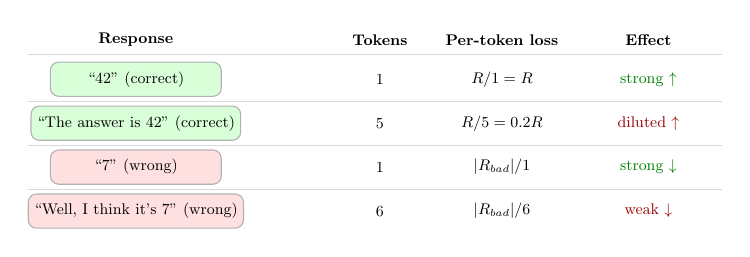
\begin{tikzpicture}[
      scale=0.62, every node/.style={scale=0.62},
      box/.style={rectangle, draw=gray!60, rounded corners=3pt, minimum height=0.7cm, align=center, font=\small},
    ]
      % Header
      \node[font=\small\bfseries] at (0, 2.8) {Response};
      \node[font=\small\bfseries] at (5, 2.8) {Tokens};
      \node[font=\small\bfseries] at (7.5, 2.8) {Per-token loss};
      \node[font=\small\bfseries] at (10.5, 2.8) {Effect};

      % Row 1: Short correct
      \node[box, fill=green!15, minimum width=3.5cm] at (0, 2) {``42'' (correct)};
      \node[font=\small] at (5, 2) {1};
      \node[font=\small] at (7.5, 2) {$R / 1 = R$};
      \node[font=\small, text=green!50!black] at (10.5, 2) {strong $\uparrow$};

      % Row 2: Long correct
      \node[box, fill=green!15, minimum width=3.5cm] at (0, 1.1) {``The answer is 42'' (correct)};
      \node[font=\small] at (5, 1.1) {5};
      \node[font=\small] at (7.5, 1.1) {$R / 5 = 0.2R$};
      \node[font=\small, text=red!60!black] at (10.5, 1.1) {diluted $\uparrow$};

      % Row 3: Short wrong
      \node[box, fill=red!12, minimum width=3.5cm] at (0, 0.2) {``7'' (wrong)};
      \node[font=\small] at (5, 0.2) {1};
      \node[font=\small] at (7.5, 0.2) {$|R_\text{bad}| / 1$};
      \node[font=\small, text=green!50!black] at (10.5, 0.2) {strong $\downarrow$};

      % Row 4: Long wrong
      \node[box, fill=red!12, minimum width=3.5cm] at (0, -0.7) {``Well, I think it's 7'' (wrong)};
      \node[font=\small] at (5, -0.7) {6};
      \node[font=\small] at (7.5, -0.7) {$|R_\text{bad}| / 6$};
      \node[font=\small, text=red!60!black] at (10.5, -0.7) {weak $\downarrow$};

      % Divider lines
      \draw[gray!30] (-2.2, 2.5) -- (12, 2.5);
      \draw[gray!30] (-2.2, 1.55) -- (12, 1.55);
      \draw[gray!30] (-2.2, 0.65) -- (12, 0.65);
      \draw[gray!30] (-2.2, -0.25) -- (12, -0.25);
    \end{tikzpicture}
  \end{center}
  \textbf{Fix:} normalize by a constant $T_\text{max}$ instead of $|o_i|$ (next slides).
\end{frame}

% -----------------------------------------------------------------------
\begin{frame}{Dr.\ GRPO: Std.\ Normalization Bias}
  GRPO standardizes rewards \emph{within} each question's group of $G$ responses,
  $A_i = (R_i - \bar R)/{\color{red!70!black}\sigma_G}$ with $\sigma_G = \operatorname{std}(\{R_1,\dots,R_G\})$, so $1/\sigma_G$ acts as a \emph{per-question} weight on the whole group's gradient.
  \vspace{-0.2em}
  \begin{itemize}\setlength{\itemsep}{0.1em}
    \item \textbf{Nearly-solved} (or nearly-impossible): almost all $R_i$ equal $\Rightarrow$ $\sigma_G\!\to\!0$ $\Rightarrow$ $1/\sigma_G$ \emph{blows up}. Balanced, \emph{informative} problems (large $\sigma_G$) get \emph{down}-weighted. Binary rewards: $\sigma_G\!\approx\!\sqrt{p(1-p)}$.
    \item[$\Rightarrow$] A rare deviation on an easy problem gets a far stronger gradient than any answer on a genuinely hard (balanced) problem.
  \end{itemize}
  \vspace{-0.1em}
  \begin{center}
  \resizebox{0.98\textwidth}{!}{%
    \begin{tikzpicture}[
      dot/.style={circle, draw=gray!50, minimum size=4mm, inner sep=0pt, font=\scriptsize},
      correct/.style={dot, fill=green!25},
      wrong/.style={dot, fill=red!25},
    ]
      % ---- Panel A: nearly solved ----
      \node[font=\bfseries] at (2.1,2.7) {Nearly solved};
      \node[font=\scriptsize\itshape] at (2.1,2.35) {7/8 correct};
      \foreach \i in {1,...,7} { \node[correct] at ({0.55*\i},1.7) {1}; }
      \node[wrong] at ({0.55*8},1.7) {0};
      \node[font=\scriptsize] at (2.1,1.0) {$\bar R=0.875,\ \sigma_G=0.33$ {\footnotesize(small)}};
      \node[font=\scriptsize, anchor=east] at (0.2,0.2) {$A$};
      \draw[gray!40] (0.4,0.2) -- (4.6,0.2);
      \draw[red!70!black, line width=2.2pt, -{Stealth}] (0.55*8,0.2) -- (0.55*8,-1.1)
         node[midway, right=1pt, font=\scriptsize, text=red!70!black] {$-2.6$};
      \draw[green!50!black, line width=2.2pt, -{Stealth}] (2.0,0.2) -- (2.0,0.48)
         node[right=1pt, font=\scriptsize, text=green!50!black] {$+0.4$};

      % ---- Panel B: medium (x offset +5.4) ----
      \begin{scope}[xshift=5.4cm]
        \node[font=\bfseries] at (2.1,2.7) {Medium difficulty};
        \node[font=\scriptsize\itshape] at (2.1,2.35) {4/8 correct};
        \foreach \i in {1,...,4} { \node[correct] at ({0.55*\i},1.7) {1}; }
        \foreach \i in {5,...,8} { \node[wrong] at ({0.55*\i},1.7) {0}; }
        \node[font=\scriptsize] at (2.1,1.0) {$\bar R=0.5,\ \sigma_G=0.50$ {\footnotesize(large)}};
        \node[font=\scriptsize, anchor=east] at (0.2,0.2) {$A$};
        \draw[gray!40] (0.4,0.2) -- (4.6,0.2);
        \draw[red!70!black, line width=2.2pt, -{Stealth}] (3.6,0.2) -- (3.6,-0.3)
           node[midway, right=1pt, font=\scriptsize, text=red!70!black] {$-1.0$};
        \draw[green!50!black, line width=2.2pt, -{Stealth}] (1.4,0.2) -- (1.4,0.7)
           node[right=1pt, font=\scriptsize, text=green!50!black] {$+1.0$};
      \end{scope}

      % ---- Panel C: 1/sigma curve (right) ----
      \begin{axis}[
          at={(11.6cm,-1.2cm)},
          width=5.6cm, height=4.6cm,
          xlabel={success rate $p$}, ylabel={weight $1/\sigma_G$},
          domain=0.06:0.94, samples=100,
          xmin=0, xmax=1, ymin=0, ymax=4.5,
          xtick={0,0.5,1}, ytick={2,4},
          axis lines=left, tick align=outside,
          every axis label/.style={font=\scriptsize},
          tick label style={font=\scriptsize}, clip=false,
        ]
        \addplot[vir2, line width=1.3pt] {1/sqrt(x*(1-x))};
        \node[font=\scriptsize, red!70!black] at (axis cs:0.17,3.9) {easy};
        \node[font=\scriptsize, red!70!black] at (axis cs:0.80,3.9) {hard};
        \node[font=\scriptsize, green!50!black] at (axis cs:0.5,1.35) {informative};
        \draw[green!50!black, -{Stealth}] (axis cs:0.5,1.6) -- (axis cs:0.5,1.92);
        \fill[red!70!black] (axis cs:0.1,3.33) circle (1.4pt);
        \fill[red!70!black] (axis cs:0.9,3.33) circle (1.4pt);
        \fill[green!50!black] (axis cs:0.5,2.0) circle (1.4pt);
      \end{axis}
    \end{tikzpicture}%
  }
  \end{center}
  \vspace{-0.2em}
  \textbf{Fix:} drop the $\sigma_G$ division, $A_i = R_i - \bar R$, so every question contributes on the same scale.
\end{frame}

% -----------------------------------------------------------------------
\begin{frame}{Dr.\ GRPO: Algorithm}
  \begin{algorithm}[H]
  \small
  \caption{Dr.\ GRPO (modifications in {\color{red!70!black} red})}
  \For{$k = 0$ \KwTo $K-1$}{
    \textbf{Data Collection:} Sample prompts $\{s_j\}_{j=1}^{M}$. For each $s_j$, generate $K_j$ responses using $\pi_{\theta_k}$\;
    \textbf{Reward Evaluation:} For each response $a_{jk}$, compute $R_{jk} = R(s_j, a_{jk})$\;
    \textbf{Advantage Computation:}\;
    \Indp
      Mean reward: $\bar{R}_j = \frac{1}{K_j}\sum_{k=1}^{K_j} R_{jk}$\;
      Advantage: $A_{jk} = {\color{red!70!black} R_{jk} - \bar{R}_j}$ \quad {\color{red!70!black}\scriptsize (no $\sigma$ division)}\;
    \Indm
    \textbf{Policy Update:}\;
    \Indp
      Ratio: $r_{jk,t} = \frac{\pi_\theta(a_{jk,t} \mid s_j, a_{jk,<t})}{\pi_{\theta_k}(a_{jk,t} \mid s_j, a_{jk,<t})}$\;
      $L = -{\color{red!70!black}\frac{1}{T_{\max}}} \sum_{j,k} \sum_t \min(r_{jk,t}\, A_{jk},\; \text{clip}(r_{jk,t}, 1{-}\epsilon, 1{+}\epsilon)\, A_{jk})$ \quad {\color{red!70!black}\scriptsize (fixed normalization)}\;
    \Indm
  }
  \end{algorithm}
  \vspace{0.3em}
  \begin{itemize}[nosep]
    \item {\color{red!70!black} No $\sigma_G$ division}: removes disproportionate updates on nearly-solved problems
    \item {\color{red!70!black} $T_{\max}$ normalization}: divides by max token count, not actual length $\Rightarrow$ no length bias
  \end{itemize}
\end{frame}

% -----------------------------------------------------------------------
\begin{frame}{DAPO: Decoupled Alignment Policy Optimization}
  DAPO \cite{yu2025dapo} addresses four issues in GRPO:

  \begin{description}[nosep]
    \item[Decoupled Clipping:] Symmetric clip $[1{-}\epsilon, 1{+}\epsilon]$ prevents exploration.
      DAPO uses \emphdef{asymmetric} bounds:
      \[
        \text{clip}(r_t,\; 1 - \epsilon_\text{low},\; 1 + \epsilon_\text{high}), \quad \epsilon_\text{low} = 0.2,\; \epsilon_\text{high} = 0.28
      \]
      Higher upper bound $\Rightarrow$ low-probability tokens can increase more freely.
    \item[Dynamic Sampling:] Skip prompts where all $G$ responses are all-correct or all-wrong (advantage $= 0$, wasted compute). Resample until batch has non-trivial signal.
    \item[Token-Level Averaging:] GRPO averages per-sequence ($\frac{1}{|o_i|}$), then across sequences ($\frac{1}{G}$).
      A 1-token wrong answer gets the \emphdef{same weight} as a 100-token reasoning chain.
      DAPO weights every token equally: $\frac{1}{\sum_{i=1}^G |o_i|} \sum_{i} \sum_{t} (\cdots)$.
      Longer sequences contribute proportionally more gradient.
      (Compare Dr.\ GRPO's $T_\text{max}$ fix: different approach to the same length bias.)
    \item[No KL Penalty:] For long chain-of-thought reasoning, KL to $\pi_\text{ref}$ is counterproductive. DAPO drops it entirely.
  \end{description}
\end{frame}

\subsection{DPO}

% -----------------------------------------------------------------------
\begin{frame}{DPO: Direct Preference Optimization}
  Recall the \emphdef{Bradley-Terry model} \cite{rafailov2024dpo}:
  \[
    P(y_w \succ y_l) = \frac{\exp r(x, y_w)}{\exp r(x, y_w) + \exp r(x, y_l)}
  \]

  The RLHF overall objective:
  \[
    \max_{\pi_\theta} \E_{x \sim D, y \sim \pi_\theta(\cdot|x)}[r(x, y)] - \beta\,\text{KL}[\pi_\theta(x, y) \| \pi_\text{ref}(y \mid x)]
  \]

  \begin{itemize}
    \item Difficult: Non-differentiable, many moving parts, RL setting
    \item \emphdef{DPO Idea:} Put away with reward model and RL-loop, directly optimize a preference based loss formulated as maximum likelihood
  \end{itemize}
\end{frame}

% -----------------------------------------------------------------------
\begin{frame}{The Optimal Policy}
  \textbf{RLHF objective:}
  \[
    \max_{\pi} \E_{x, y \sim \pi(\cdot|x)}[r(x, y)] - \beta\,\text{KL}[\pi(y \mid x) \| \pi_\text{ref}(y \mid x)]
  \]

  \textbf{Optimal policy:}
  \[
    \pi^*(y \mid x) = \frac{1}{Z(x)} \pi_\text{ref}(y \mid x) \exp\!\left(\tfrac{1}{\beta}\,r(x, y)\right)
  \]
  where $Z(x) = \sum_y \pi_\text{ref}(y \mid x) \exp\!\left(\frac{1}{\beta}\,r(x, y)\right)$ is the partition function.

  \vspace{0.5em}
  Since KL is nonnegative and achieves its unique minimum when both distributions are equal, the optimal policy $\pi^*$ uniquely minimizes the objective.
\end{frame}

% -----------------------------------------------------------------------
\begin{frame}{The Optimal Policy: Reward in Terms of Policy}
  Rearrange to express the reward:
  \[
    r(x, y) = \beta \log \frac{\pi^*(y \mid x)}{\pi_\text{ref}(y \mid x)} + \beta \log Z(x)
  \]

  Plug into the Bradley-Terry model:
  \[
    P(y_w \succ y_l) = \sigma\!\left(\beta \log \frac{\pi^*(y_w \mid x)}{\pi_\text{ref}(y_w \mid x)} - \beta \log \frac{\pi^*(y_l \mid x)}{\pi_\text{ref}(y_l \mid x)}\right)
  \]
  Note: the partition functions $Z(x)$ cancel out!

  \vspace{0.5em}
  \textbf{DPO Loss:}
  \[
    \boxed{\mathcal{L}_\text{DPO}(\theta; \pi_\text{ref}) = -\E_{(x,y_w,y_l) \sim D}\!\left[\log \sigma\!\left(\beta \log \frac{\pi_\theta(y_w \mid x)}{\pi_\text{ref}(y_w \mid x)} - \beta \log \frac{\pi_\theta(y_l \mid x)}{\pi_\text{ref}(y_l \mid x)}\right)\right]}
  \]
  Optimizing $\mathcal{L}_\text{DPO}$ w.r.t.\ $\theta$ $\Rightarrow$ obtaining optimal policy $\pi^*$.
\end{frame}

\subsection{Summary and Open Problems}

% -----------------------------------------------------------------------
\begin{frame}{Open Research Challenges}
  \begin{description}\largesep
    \item[Credit Assignment:] Current outcome-based methods assign essentially the same reward to all tokens. This works but is inefficient. Process reward models and step-level verifiers remain unsolved.
    \item[Sample Efficiency:] Methods require 8--64 rollouts per prompt despite information being just a single bit (correct/incorrect).
    \item[Very Hard Problems:] No gradient signal when models never produce correct rollouts. Curriculum learning provides only workarounds.
    \item[Domain Generalization:] Progress concentrates in domains with cheap and unambiguous verification (math and code). Extending to noisy or subjective evaluation remains difficult.
    \item[Empirical Reliability:] Evidence remains relatively narrow and expensive to reproduce.
    \item[New Capabilities vs.\ Distribution Narrowing:] Does RL teach fundamentally new skills, or does it merely \emphdef{sharpen the output distribution} toward abilities already latent from pretraining? Evidence suggests RL primarily surfaces and focuses existing capabilities rather than creating novel ones. The ceiling may be set by pre- and mid-training.
  \end{description}
\end{frame}

% -----------------------------------------------------------------------
\begin{frame}{Policy Gradient Intuition}
  \begin{center}
    
\includegraphics[width=0.85\textwidth]{images/rl_meme.png}
  \end{center}
\end{frame}
